\chapter{面向 Aloha 协议的连续传输机制设计与性能分析}
\label{chapter3:SAST}

上一章分析了 5G 随机接入标准框架。尽管其包含复杂的信令与协议过程，但在 2 步小数据传输场景下，可将接入过程抽象为时隙 Aloha 模型。基于此，本章回到抽象模型，在统一假设下分析接入竞争与连续传输机制。在此基础上，提出连续传输增强的时隙 Aloha 机制，即 SAST ，并依次给出机制流程、休假排队建模以及吞吐量与时延性能分析。 

\section{SAST系统模型与机制描述}
\label{sec:sast_system_model}

本章所研究的 SAST 网络环境遵循~\ref{sec:general_system_model}~节定义的通用系统模型。具体而言，考虑由 $n$ 个同质节点和单个接收机构成的分布式时隙 Aloha 网络，节点流量服从伯努利到达，信道采用碰撞模型，且具备即时无误的确认或否定确认反馈机制。

SAST 协议的核心策略可以概括为一次接入、连续占用，可打破传统 Aloha 协议中每发送一个数据包都需重新竞争的低效模式。具体而言，当节点缓存非空时，首先以概率 $q \in [0,1]$ 参与随机竞争并传输队首数据包。若接收机成功解码该数据包，则回复确认消息，节点随即进入连续传输阶段；若发生碰撞或解码失败，则回复否定确认消息，节点在下一时隙重新以概率 $q$ 尝试接入。一旦队首数据包成功传输，该节点便可视为获得了短时信道占用权。在后续若干时隙内，该节点不再进行随机退避，而是以概率 1 连续发送缓存中的剩余数据包，直到缓存清空或发生信道碰撞。

为了直观展示这一过程，图~\ref{fig:two_node_sast} 以两个节点为例，描绘了 SAST 网络中典型的竞争、连续传输及中断过程：
\begin{figure}[t]
	\centering
	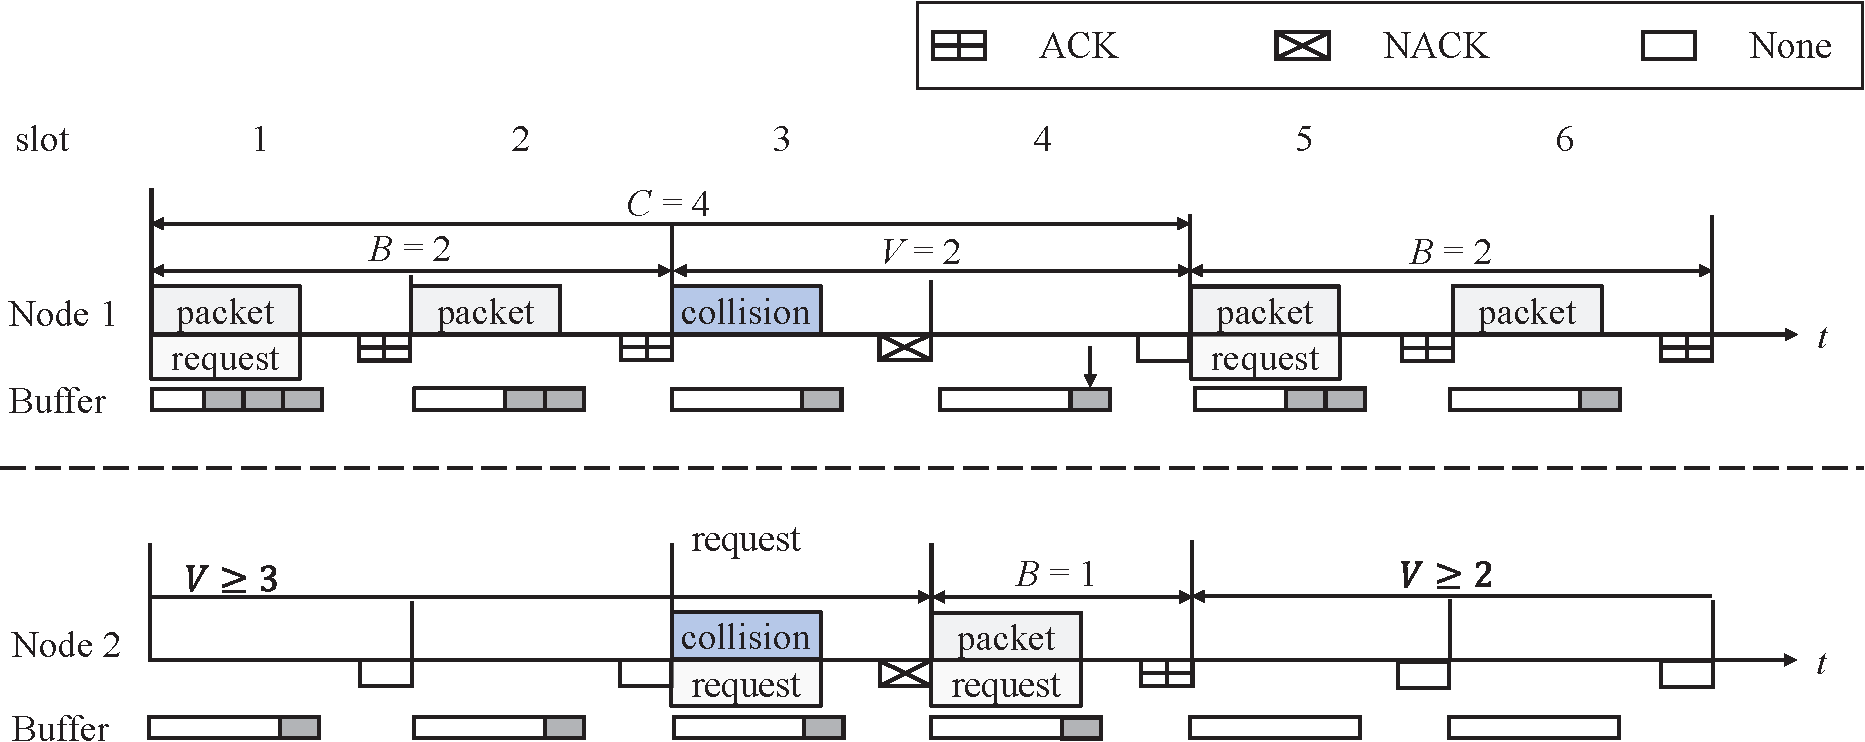
\includegraphics[width=0.9\textwidth]{figure/chap3/two_node_sast.pdf}
	\caption{两节点 SAST 网络时序示意图}
	\label{fig:two_node_sast}
\end{figure}
\begin{description}
	\item[时隙 1 （初始接入）：] 节点 1 以概率 $q$ 成功发送队首数据包，而节点 2 保持静默。节点 1 收到确认反馈后进入连续传输状态。
	\item[时隙 2 （连续传输）：] 节点 1 无需再次竞争，直接以概率 1 发送缓存中的第二个数据包并成功。
	\item[时隙 3 （碰撞中断）：] 节点 1 试图发送第三个数据包。与此同时，节点 2 恰好到达新数据包并以概率 $q$ 发起队首包传输。两者信号叠加引发碰撞，基站回复否定确认。此次碰撞强制中止了节点 1 的连续传输过程，使其退回常规竞争状态。
	\item[时隙 4 （重新竞争）：] 网络恢复到无节点占用的状态。节点 1 和节点 2 重新参与信道竞争，此时节点 2 以概率 $q$ 成功抢占信道发送队首包，而节点 1 保持静默。
\end{description}

需要特别指出的是，本章所提出的 SAST 机制在思想上虽与传统基于连接的 Aloha 或 5G 中的免调度均体现出一定的连续占用特征，但在设计范式存在本质区别。现有机制通常依赖显式预约或连接建立过程来实现信道的持续占用，SAST 采用的是一种隐式预留策略：节点无需发送专门的 RTS/RRC 等额外控制信令，而是用 5G 标准中的 MsgA 报文进行竞争；一旦基站成功解码并反馈 MsgB，后续信道占用通过连续发送数据报文自然延续，该过程是不改变现有分布式接入架构与帧结构的。
为避免与其他 Aloha 类协议混淆，这里从机制实现角度对三类 Aloha 协议作简要总结，如表~\ref{tab:aloha_compare} 所示。

\begin{table}[htbp]
\centering
\caption{SA、CBA 与 SAST 机制的核心特性对比}
\label{tab:aloha_compare}
\renewcommand{\arraystretch}{1.3} 
\begin{tabular}{l c c c}
\toprule
\textbf{对比维度} & \textbf{SA} & \textbf{CBA} & \textbf{SAST（本文）} \\
\midrule
接入机制 & 逐包独立竞争 & 显式信令预约 & 隐式预留 (复用 MsgA) \\
连续传输 & 不支持 & 静态配置 (固定 $M$) & 动态自适应 (队列驱动) \\
释放条件 & 单包传毕即放 & 预留期满释放 & 队列清空或遭遇碰撞 \\
连接管理 & 无连接态 & 需建立与维护连接 & 无连接态 \\
信令开销 & 基础反馈 & 高 (需控制信令交互) & 基础反馈 \\
中断机制 & 不适用 & 预留期内不可打断 & 碰撞即时中断并退避 \\
\bottomrule
\end{tabular}
\end{table}

\section{基于休假排队理论的系统建模}
\label{sec:sast_queuing_model}

为深入量化分析 SAST 机制的性能，本节引入离散时间休假排队理论\cite{2021_Huang}，分别从节点和信道两个互补视角对系统行为进行建模。这种建模方法能够有效地将节点的数据包到达过程与信道的传输竞争过程解耦，从而通过分析忙期与假期的统计特性推导系统的吞吐量与时延性能。

%\subsection{节点视角的休假队列模型}
\label{subsec:node_perspective}

从节点视角出发，节点在长期运行过程中可抽象为两个交替出现的阶段，即节点忙期 $B$ 与节点假期 $V$。其中，忙期 $B$ 指节点成功占用信道后以连续传输方式发送数据包的时间段。由于本章采用离散时隙模型，并以成功接入作为忙期触发事件，因此忙期 $B$ 的计数从队首数据包成功传输所在的时隙开始，从而 $B\ge 1$。随后节点进入连续传输阶段，在后续时隙中以概率 1 发送队列中的剩余数据包，直至缓存清空或发生碰撞时结束。假期 $V$ 则表示节点未能完成成功数据传输的时间段，主要包括三类情形：缓存为空、缓存非空但未发起接入，以及发起接入但发生碰撞。此外，定义节点周期 $C$ 为相邻两次忙期起始时刻之间的时间间隔，因此有 $C = B + V$。

从信道视角来看，其运行状态同样呈现出周期性交替特征。定义信道忙期 $B_c$、信道假期 $V_c$ 和信道周期 $C_c$。其中，信道忙期 $B_c$ 指信道被任意一个节点成功占用并进行数据传输的时间段，信道假期 $V_c$ 指信道上没有数据包被成功解码的时间段，即信道处于空闲状态或发生碰撞，信道周期 $C_c$ 为两个连续信道忙期起始点之间的时间间隔，即 $C_c = B_c + V_c$。
值得注意的是，由于信道忙期 $B_c$是由任意一个节点的成功接入所触发的，因此信道忙期 $B_c$ 的概率分布与单个节点的忙期 $B$ 完全一致。为简化符号，后续分析中将统一使用 $B$ 来表示忙期。

基于上述休假排队模型的符号定义，网络的接入吞吐量 $\lambda^a_{out}$和数据吞吐量 $\lambda^d_{out}$可由信道周期的统计特性推导定义。
由于在一个信道周期 $C_c$ 内，仅有一次成功的接入请求，即触发该忙期的队首数据包，接入吞吐量定义为成功接入次数与周期长度之比：
\begin{equation}
	\lambda^a_{out} = \frac{1}{\bar{C}_c} = \frac{1}{\bar{B} + \bar{V}_c}.
	\label{eq:access_throughput_def}
\end{equation}
另一方面，数据吞吐量定义为信道处于传输有效数据状态的时间比例，即平均忙期长度与周期长度之比：
\begin{equation}
	\lambda^d_{out} = \frac{\bar{B}}{\bar{C}_c} = \frac{\bar{B}}{\bar{B} + \bar{V}_c}.
	\label{eq:data_throughput_def}
\end{equation}
其中，$\bar{X}$ 表示随机变量 $X$ 的期望值（均值）。接下来的分析重点将在于如何根据系统参数（如节点数 $n$、传输概率 $q$）推导 $\bar{B}$ 和 $\bar{V}_c$ 的闭式解。


\subsection{信道休假队列分析}
\label{subsec:channel_vacation_analysis}

在对 SAST 系统的性能进行详细推导之前，首先需要对信道上的聚合请求业务流进行统计建模。令随机变量 $\Theta$ 表示在信道上任意一个空闲时隙内产生的接入请求总数。该变量聚合了系统中所有节点新生成的数据包请求以及积压的重传请求。
记 $\theta = \mathbb{E}[\Theta]$ 为 $\Theta$ 的数学期望，即系统的尝试速率。
考虑到网络中存在 $n$ 个同质节点，在任意时隙开始时，设每个节点的缓存非空概率为 $p_{ne}$。
根据 SAST 机制的设计，只有当节点缓存非空时，其才会以概率 $q$ 发起接入尝试，即发送队首数据包；否则节点保持静默。
因此，对于整个网络而言，该时隙内的并发接入请求数量 $\Theta$ 实际上服从参数为 $(n, q p_{ne})$ 的二项分布：
\begin{equation}
	\Pr \{\Theta = i\} = C_n^i (q p_{ne})^i (1 - q p_{ne})^{n-i}, \quad i = 0, 1, \dots, n.
\end{equation}

在典型的物联网场景中，通常满足节点数量 $n$ 较大且单节点传输概率 $q$ 较小的特征。
根据极限定理，上述二项分布可以近似为参数为 $\theta$ 的泊松分布\footnote{泊松近似在海量随机接入系统的性能分析中被广泛采用，其有效性已在多篇文献中得到验证。}。
此时，接入请求数量的概率质量函数可表示为：
\begin{equation}
	\label{eq:poisson_prob}
	\Pr \{\Theta = i\} \approx \frac{e^{-\theta} \theta^i}{i!}, \quad i = 0, 1, \dots, \infty,
\end{equation}
其中，尝试速率 $\theta$ 由下式给出：
\begin{equation}
	\label{eq:theta_general}
	\theta = n q p_{ne}.
\end{equation}
当网络处于饱和状态时，节点缓存始终非空，即 $p_{ne} = 1$，此时尝试速率简化为 $\theta_{sa} = nq$；当网络处于非饱和状态时，节点缓存可能为空，即 $0 < p_{ne} < 1$，此时尝试速率 $\theta$ 取决于系统的稳态运行点。基于此泊松近似模型，我们将在下文中利用尝试速率 $\theta$，分别推导信道假期和信道忙期的统计特性。

先讨论信道假期平均长度 $\overline{V}_c$。根据 SAST 机制，当信道处于假期时，所有积压节点会在每个时隙以竞争方式尝试接入。基于前述的泊松近似，在任意时隙内，恰好有一个节点发送请求的概率为 $\theta e^{-\theta}$；反之，没有节点发送或多个节点发送的概率为 $1 - \theta e^{-\theta}$。另一方面，由于每个时隙的竞争结果相互独立，信道从假期状态转变为忙期状态的过程可视为一系列独立的伯努利试验，直至出现第一次成功接入。这决定了假期的持续时间本质上服从参数为 $\theta e^{-\theta}$ 的几何分布。具体分布形式取决于上一个忙期的结束方式，可归纳为以下两种情形：
\begin{itemize}
	\item 情形一对应缓存清空触发。当前占用信道的节点成功发送完所有数据包后，缓存清空并主动释放信道。此时，信道在当前时隙结束后立即对所有节点可用。若在紧接着的下一个时隙立即发生一次成功接入，概率为 $\theta e^{-\theta}$，则信道无缝切换至下一个忙期，物理上的假期时间为 0。因此，该情形下 $V_c$ 服从定义域包含 0 的几何分布：
	\begin{equation}
		\Pr \{ V_c = i \mid \text{情形1} \} = (1 - \theta e^{-\theta})^i \theta e^{-\theta}, \quad i = 0, 1, \ldots
	\end{equation}
	
	\item 情形二对应碰撞中断触发。当前忙期由于节点在传输过程中遭遇其他节点的并发传输而被迫中止。值得注意的是，发生碰撞的那个时隙本身既没有成功传输数据，也无法被利用，因此该时隙必须计入随后的假期中。这意味着，即使在碰撞后的下一个时隙立即成功接入，假期总长度也至少为 1。因此，该情形下 $V_c$ 服从定义域从 1 开始的移位几何分布：
	\begin{equation}
		\Pr \{ V_c = i \mid \text{情形2} \} = (1 - \theta e^{-\theta})^{i-1} \theta e^{-\theta}, \quad i = 1, 2, \ldots
	\end{equation}

\end{itemize}
综合上述两种情形，并利用几何分布的期望性质，可推导得到信道假期的平均长度 $\overline{V}_c$ 为：
\begin{equation}
	\label{eq:mean_vc_derived}
	\overline{V}_c = p_0 \underbrace{\frac{1 - \theta e^{-\theta}}{\theta e^{-\theta}}}_{\mathbb{E}[V_c \mid \text{情形1}]} + (1 - p_0) \underbrace{\frac{1}{\theta e^{-\theta}}}_{\mathbb{E}[V_c \mid \text{情形2}]} = \frac{e^{\theta}}{\theta} - p_0,
\end{equation}
其中 $p_0$ 表示节点在一个忙期内清空缓存的概率，该关键参数由后续分析给出。


接下来，我们将分析信道忙期平均长度 $\overline{B}$。与假期取决于竞争何时成功不同，忙期持续时间取决于传输何时被中断或数据缓存何时被传输完毕。这一过程直接受限于网络或节点的负载状态，因此也分两种情况讨论：
\begin{itemize}
	\item 非饱和情况： 
	当网络处于非饱和状态时，网络下节点的数据队列可能为空。此时，忙期既可能因碰撞结束，也可能因节点发完数据（$p_0 > 0$）而结束，其分布较为复杂。
	为简化推导，我们利用网络流量守恒定理进行说明。在稳态下，系统能够及时处理所有到达的业务流量，即系统的平均数据吞吐量 $\lambda_{out}^d$ 必须等于网络的聚合输入速率 $\hat{\lambda} = n\lambda$。
	回顾前述数据吞吐量的定义式 $\lambda_{out}^d = \frac{\overline{B}}{\overline{B} + \overline{V}_c}$，我们有：
	\begin{equation}
		\frac{\overline{B}_{unsa}}{\overline{B}_{unsa} + \overline{V}_c} = \hat{\lambda}.
	\end{equation}
	通过代数变换，可直接反解出非饱和情况下的平均忙期长度，建立其与信道假期 $\overline{V}_c$ 的线性关系：
	\begin{equation}
		\overline{B}_{unsa} = \frac{\hat{\lambda}}{1 - \hat{\lambda}} \overline{V}_c.
	\end{equation}

	\item 饱和情况： 
	在此状态下，假设网络处于重负载，所有节点缓存始终非空（即 $p_{ne}=1$），这意味着节点永远不会因为没数据发而主动释放信道，同时也可以推断出缓存清空概率 $p_0 = 0$，尝试速率恒定为 $\theta_{sa} = nq$。
	
	根据 SAST 机制，一旦节点进入忙期，它将以概率 1 连续发送数据包。该过程仅在发生碰撞时被迫终止。在忙期内的任意时隙，除当前传输节点外的其他 $n-1$ 个节点均可能发起接入。基于泊松近似，该时隙未发生碰撞的概率为 $e^{-\theta_{sa}}$，发生碰撞（即至少有一个其他节点接入）的概率为 $1 - e^{-\theta_{sa}}$\footnote{这里认为当节点数量$n$很大的时候，$n-1$近似为$n$。}。
	由于每个时隙的碰撞事件相互独立，忙期的维持过程同样可视为一系列参数为 $1 - e^{-\theta_{sa}}$ 的伯努利试验。因此，饱和忙期长度 $\overline{B}_{sa}$ 服从几何分布，其均值为碰撞概率的倒数：
	\begin{equation}
		\overline{B}_{sa} = \frac{1}{1 - e^{-\theta_{sa}}} = \frac{1}{1 - e^{-nq}}.
	\end{equation}
	

\end{itemize}

通过上述信道视角的分析，我们成功推导了 $\overline{V}_c$ 和 $\overline{B}$ 的表达式。然而，可以观察到这些表达式均依赖于关键参数：尝试速率 $\theta$（或等价为节点缓存非空概率 $p_{ne}$以及忙期内缓存清空概率 $p_0$）。这些参数由节点内部的数据包到达以及节点数据服务过程所决定。为获得闭式解，我们需要进一步从节点视角对休假排队模型进行分析。


\subsection{节点休假队列分析}

\label{subsec:node_vacation_analysis}

前一小节已经表明，系统性能的关键在于尝试速率 $\theta$ 与缓存清空概率 $p_0$。为进一步确定这两个参数，本节将分析视角由信道转向节点，重点刻画单节点休假排队过程及其队列长度演化规律。从节点层面看，其运行过程仍然可被视为忙期 $B$ 与假期 $V$ 的交替循环。而队列长度的变化则由数据包到达与服务过程共同决定。基于此，本文定义 $A_B$ 为节点在一个忙期内的新到达包数，$A_V$ 为节点在一个假期内的新到达包数。下面将分别推导二者的统计分布。

先分析忙期内到达过程 $A_B$。当一个节点处于忙期时，其正在连续传输数据包。在此期间，新数据包的到达服从参数为 $\lambda$ 的伯努利过程。
为了推导忙期内到达数 $A_B$ 的统计特性，我们采用概率生成函数的方法。首先，假设忙期长度固定为 $j$ 个时隙，即 $B=j$。由于每个时隙的数据包到达相互独立，该段时间内的到达总数服从参数为 $(j, \lambda)$ 的二项分布，其条件概率生成函数可表示为 $ \mathbb{E}[z^{A_B} \mid B=j] = (\lambda z + 1 - \lambda)^j $。利用全概率公式，对忙期长度 $B$ 的所有可能取值进行加权求和，可得到 $A_B$ 的无条件概率生成函数：
	$ G_{A_B}(z) = \sum_{j=1}^{\infty} \Pr \{B = j\} (\lambda z + 1 - \lambda)^j $。
观察上式形式，根据 $G_B(z) = \sum \Pr\{B=j\} z^j$ 的定义，可以发现 $G_{A_B}(z)$ 本质上是忙期长度概率生成函数PGF的复合函数：
\begin{equation}
	\label{eq:G_AB_exact}
	G_{A_B}(z) = G_B(\lambda z + 1 - \lambda).
\end{equation}

虽然式 (\ref{eq:G_AB_exact}) 给出了准确表达式，但在复杂的排队分析中直接求解较为困难。考虑到在大规模物联网场景中，节点数量 $n$ 较大，而系统总负载有限，因此单个节点的输入速率 $\lambda$ 通常为一个远小于1的量，即 $\lambda \ll 1$。基于此特性，我们可以对 $G_{A_B}(z)$ 在 $z=1$ 附近进行一阶泰勒展开近似。令 $y = \lambda z + 1 - \lambda$，当 $\lambda \to 0$ 时，$y \to 1$。根据 PGF 的性质 $G_B(1)=1$ 且 $G_B'(1)=\overline{B}$，我们有：
\begin{equation}
	\begin{aligned}
		G_{A_B}(z) & \approx G_B(1) + G_B'(1)(y - 1) + o(\lambda) \\
		& = 1 + \overline{B} (\lambda z - \lambda) + o(\lambda) \\
		& = 1 - \lambda \overline{B} + \lambda \overline{B} z.
	\end{aligned}
	\label{eq:G_AB_approx}
\end{equation}
这一近似结果具有明确的物理意义：在单节点低负载条件下，一个忙期内到达的数据包数量主要集中在 0 个或 1 个。具体而言，式中常数项 $1 - \lambda \overline{B}$ 近似表示忙期内没有新包到达的概率，而一次项系数 $\lambda \overline{B}$ 近似表示忙期内恰好到达 1 个新包的概率。忽略高阶项即到达 2 个及以上数据包的情况，极大简化了后续稳态分布的求解过程。


再分析假期内到达过程 $A_V$。当忙期结束时，节点切换至假期 $V$。根据假期开始时刻节点缓存状态的不同，节点的行为模式可分为两类。我们分别定义 $A_{V_1}$ 和 $A_{V_0}$ 为这两类假期内的数据包到达数量：
\begin{itemize}
	\item 类型 1 假期对应非空启动。这种情况发生在上一忙期因碰撞而被迫中断时，假期开始时刻节点缓存非空。此时，节点无需等待，立即参与信道竞争。其持续时间等同于从发起请求到成功接入的等待时间。基于节点在每一时隙的竞争成功概率 $q e^{-\theta}$，我们可以推导出 $A_{V_1}$ 的 PGF 为：
	\begin{equation}
		\label{eq:G_AV1}
		G_{A_{V_1}}(z) = \frac{q e^{-\theta} (1 - \lambda + \lambda z)}{1 - [1 - q e^{-\theta} + (G_{A_B}(z) - 1)(1 - q) \theta e^{-\theta}](1 - \lambda + \lambda z)}.
	\end{equation}
	证明见附录\ref{app:proof_lemma1}。
	\item 类型 0 假期对应空启动。这种情况发生在上一忙期节点成功清空缓存时，假期开始时刻节点缓存为空。此时，节点必须处于静默状态等待新数据包到达。该过程由两部分组成：一是等待新数据包到达的时间，其服从几何分布；二是数据包到达后节点转入竞争状态，即经历一个类型 1 假期。因此，类型 0 假期的到达数恒等于类型 1 假期的到达数加 1，即触发该假期的那个新到达包，$A_{V_0} = 1 + A_{V_1}$。相应地，其 PGF 满足 $G_{A_{V_0}}(z) = z G_{A_{V_1}}(z)$。
\end{itemize}
综合上述分析，节点在一个节点假期 $V$ 内的到达数 $A_V$ 取决于节点是否清空了缓存。
% 结合缓存清空概率 $p_0$，整体到达数 $A_V$ 的 PGF 可表示为两者的加权和。
当节点数量 $n$ 很大时，$ G_{A_{V}}(z) $ 可表示为：
% \begin{equation}
% 	\label{eq:G_AV_combined}
% 	G_{A_V}(z) = (1 - p_0) G_{A_{V_1}}(z) + p_0 G_{A_{V_0}}(z) = [ (1 - p_0) + p_0 z ] G_{A_{V_1}}(z).
% \end{equation}

\begin{equation}
\label{eq:G_AV_combined}
G_{A_{V}}(z) =
\begin{cases}
	\dfrac{\beta}{1-(1-\beta) z}(1-\lambda+\lambda z)+o\left(\dfrac{1}{n}\right), & 1-p_{0} \\[10pt]
	\dfrac{\beta}{1-(1-\beta) z}(1-\lambda+\lambda z)z+o\left(\dfrac{1}{n}\right), & p_{0}
\end{cases}
\end{equation}
其中，$ p_{0} $ 表示在一个忙周期内，传输节点能够清空其缓存的概率，且
\begin{equation}
\label{eq:beta_defination}
\beta = \frac{q e^{-\theta}}{q e^{-\theta}+\lambda\left[1-q e^{-\theta}+\bar{B}(1-q)\theta e^{-\theta}\right]}.
\end{equation}
至此，我们建立了节点新包到达过程与系统参数之间的解析关系，为后续求解尝试率 $\theta$ 及缓存队列被清空概率 $p_0$ 做好铺垫。

\subsection{尝试速率$\theta$与概率$p_0$分析}
\label{subsec:attempt_rate_analysis}

在前两小节中，我们分别建立了信道和节点的休假排队模型，其性能指标的闭式解均依赖于系统的尝试速率 $\theta$ 以及节点在忙期结束时清空缓存的概率 $p_0$。本节将结合稳态排队分析，推导这两个关键参数的解析表达式，从而闭合整个分析框架。

先讨论尝试速率 $\theta$ 与缓存清空概率 $p_{0}$ 的联系。尝试速率 $\theta$ 和概率 $p_0$ 是决定忙期平均长度 $\overline{B}$、节点假期平均长度 $\overline{V}$、忙期内到达数据包数量 $A_B$ 和节点假期内到达数据包数量 $A_V$ 的关键参数。在一个完整的节点周期 $C$ 中，节点缓存被清空的事件以概率 $p_0$ 发生。一旦缓存清空，节点将保持静默直至新数据包到达。由于数据包到达服从参数为 $\lambda$ 的伯努利过程，节点的平均空闲等待时间为 $1/\lambda$ 个时隙。因此，在统计平均意义下，一个节点周期 $C$ 内缓存为空的平均时长为 $p_0 / \lambda$。由此，节点缓存非空概率 $p_{ne}$ 可视为节点处于积压状态的时间比例，即
对于非饱和网络，系统处于稳态，根据流量守恒原理，节点周期内新到达的平均数据包数量应等于该周期内成功传出的数据包数量。	$ \lambda \overline{C} = \overline{B} $。
结合尝试速率的定义 $\theta = n q p_{ne}$，可得尝试速率与忙期长度及清空概率之间的关系：
\begin{equation}
	\label{eq:theta_relation}
	\theta = n q \left( 1 - \frac{p_0}{\overline{B}} \right).
\end{equation}
上式表明，求解 $\theta$ 的关键在于确定 $\overline{B}$ 和 $p_0$。其中 $\overline{B}$ 已在前文建立了其与 $\theta$ 和 $p_0$ 的函数关系，因此问题的核心转化为求解概率 $p_0$。

接下来我们继续分析 $p_0$ 的求解及节点缓存队列的稳态分布。为得到概率 $p_0$，需要分析节点队列长度的稳态分布。令 $Q_t$ 和 $P_t$ 分别表示节点在第 $t$ 个忙期开始时刻和结束时刻的队列长度。当系统趋于稳态时，$t \to \infty$，设 $Q$ 和 $P$ 分别为对应的稳态随机变量，其概率生成函数记为 $G_Q(z)$ 和 $G_P(z)$。

一方面，根据 SAST 机制，忙期开始时的队列长度 $Q$ 由上一忙期结束时的剩余队列 $P$ 加上随后假期内新到达的数据包 $A_V$ 叠加构成。即满足线性关系 $Q = P + A_V$。为了推导 $Q$ 的概率生成函数 $G_Q(z)$，我们根据 $P$ 的状态对 $A_V$ 的分布进行条件展开：
\begin{equation}
	\begin{aligned}
		G_Q(z) &= \mathbb{E}\left[ z^{P + A_V} \right] \\
		&= \mathbb{E}\left[ z^{P + A_V} \mid P = 0 \right] \Pr\{P = 0\} + \sum_{j=1}^{\infty} \mathbb{E}\left[ z^{P + A_V} \mid P = j \right] \Pr\{P = j\}.
	\end{aligned}
\end{equation}
根据节点假期的定义，当 $P=0$ 时，节点经历类型0假期，到达数 $A_V$ 服从 $A_{V_0}$ 的分布；当 $P=j \ge 1$ 时，节点经历类型1假期，到达数 $A_V$ 服从 $A_{V_1}$ 的分布，且此时新到达过程独立于积压数量 $j$。因此上式可化简为：
\begin{equation}
	\begin{aligned}
		G_Q(z) &= z^0 G_{A_{V_0}}(z) p_0 + G_{A_{V_1}}(z) \sum_{j=1}^{\infty} z^j \Pr\{P = j\} \\
		&= p_0 G_{A_{V_0}}(z) + G_{A_{V_1}}(z) \left[ G_P(z) - p_0 \right],
	\end{aligned}
	\label{eq:GQ_GP_relation}
\end{equation}
其中队列缓存清空概率$ p_0 $可以写成另一个形式 $p_0 = \Pr\{P=0\} = G_P(0)$。同时，上式建立了忙期首尾队列分布之间的第一个耦合关系。



另一方面，忙期过程本质上是对缓存队列的服务与截断过程。从忙期开始时刻的队列 $Q$ 演变为结束时刻的队列 $P$，取决于节点的数据传输成功概率以及碰撞发生的时机。
在 SAST 机制下，一旦节点成功接入进入忙期，它将以概率 1 连续发送数据包。对于忙期内的每一个时隙，若系统中其他 $n-1$ 个节点以总体概率 $e^{-\theta}$ 保持静默，则其队列会发生变化，并且当前节点会保持在忙期；反之，若有任意其他节点发起接入导致碰撞，对应概率为 $1-e^{-\theta}$，则忙期立即强制终止，此时节点剩余的缓存队列长度即为 $P$。除此之外，我们还得考虑节点的新包到达过程，以分析节点的在忙期缓存队列长度的演变。
为准确刻画这一动态随机过程，我们构建了一个具有吸收态的马尔可夫链\cite{2008_Markov_absorb}，如图\ref{fig:absorbing_markov}所示。在该模型中，忙期内持续的数据传输状态被建模为瞬态，而碰撞导致的忙期结束事件被建模为吸收态。通过求解该马尔可夫链的转移概率矩阵及吸收概率，可以建立 $Q$ 与 $P$ 的概率生成函数之间的映射关系。
具体的数学推导过程详见附录\ref{app:proof_appendix2}。在此，我们直接给出这一关系的最终解析表达式：
\begin{equation}
	\label{eq:GP_derived}
	G_P(z) = G_Q(e^{-\theta}) + \frac{1 - e^{-\theta}}{e^{-\theta} - z} \left[ G_Q(e^{-\theta}) - G_Q(z) \right].
\end{equation}
式中，$e^{-\theta}$ 项反映了忙期在每个时隙得以延续的概率。该式与前述的式 (\ref{eq:GQ_GP_relation}) 共同构成了描述节点队列稳态分布的方程组。理论上，联立这两个方程即可通过迭代法求解出 $G_Q(z)$ 和 $G_P(z)$ 的数值解，进而确定 $p_0 = G_P(0)$。
尽管前文建立的PGF耦合方程组（式 \ref{eq:GQ_GP_relation} 和 式 \ref{eq:GP_derived}）理论上完备准确，但在大规模网络中，直接数值迭代求解计算量大，且难以直观揭示参数间的物理关联。
当网络节点数 $n$ 较大时，单节点输入速率 $\lambda = \hat{\lambda}/n$ 趋近于零。在大系统极限下，节点队列稳态分布呈明显几何分布特征，据此我们将关键结论总结为如下定理。

\begin{theorem}
	\label{thm:geometric_Q}
	当节点数量 $n$ 较大且系统处于稳态时，忙期开始时刻的节点队列长度 $Q$ 近似服从参数为 $\alpha$ 的几何分布，其概率生成函数可表示为：
	\begin{equation}
		G_Q(z) \approx \frac{\alpha z}{1 - (1 - \alpha) z}, \quad \text{其中 } \alpha = 1 - \frac{\theta}{n q}.
	\end{equation}
	基于此分布，节点在一个忙期内成功清空缓存的概率 $p_0$ 具有如下闭式解：
	\begin{equation}
		\label{eq:p0_closed_form_1}
		p_0 = \frac{1 - \frac{\theta}{n q}}{1 - \frac{\theta e^{-\theta}}{n q}}.
	\end{equation}
\end{theorem}

\begin{proof}
该定理的详细证明过程及参数 $\alpha$ 的推导详见附录\ref{app:proof_theorem_fixed_point}。
\end{proof}

定理 \ref{thm:geometric_Q} 的核心价值在于规避概率生成函数（PGF）的复杂迭代求解过程，进而简化系统稳态特性的推导流程。将式 (\ref{eq:p0_closed_form_1}) 中的稳态空闲概率 $p_0$，代入前文推导得到的信道忙期 $\overline{B}$ 与信道假期 $\overline{V}_c$ 表达式，结合非饱和状态下的流量守恒关系 $\theta = n q (1 - p_0/\overline{B})$，经代数化简后，可得到描述系统稳态工作点的核心方程，具体总结如下定理。
\begin{theorem}
	\label{thm:fixed_point_theta}
	在 SAST 网络中，系统的尝试速率 $\theta$ 是以下超越方程的根：
	\begin{equation}
		\label{eq:theta_fixed_point}
		\frac{e^{\theta}}{\theta} + \frac{\theta}{n q} - \frac{1}{n q} = \frac{1}{\hat{\lambda}},
	\end{equation}
	其中 $\hat{\lambda} = n\lambda$ 为网络的聚合输入速率，$n$ 为节点总数，$q$ 为传输概率。
\end{theorem}

\begin{proof}
% 	由流量守恒，在非饱和稳态下尝试速率 $\theta$ 满足
% \begin{equation}
% 	\theta = n q \left( 1 - \frac{p_0}{\overline{B}} \right).
% \end{equation}
利用信道忙期与信道假期的关系 $\overline{B} = \frac{\hat{\lambda}}{1 - \hat{\lambda}} \overline{V}_c$，以及信道假期公式 $\overline{V}_c = \frac{e^{\theta}}{\theta} - p_0$，我们可以将 $\overline{B}$ 表示为：
\begin{equation}
	\overline{B} = \frac{\hat{\lambda}}{1 - \hat{\lambda}} \left( \frac{e^{\theta}}{\theta} - p_0 \right).
\end{equation}

将上述 $\overline{B}$ 和 $p_0$ 的表达式代入 $\theta$ 的定义式中：
\begin{equation}
	\frac{\theta}{n q} = 1 - \frac{p_0 (1 - \hat{\lambda})}{\hat{\lambda} (\frac{e^{\theta}}{\theta} - p_0)}.
\end{equation}
经移项、通分和化简，消去 $p_0$ 的分母项。最终得到关于 $\theta$ 的隐函数方程。
\end{proof}
式 (\ref{eq:theta_fixed_point}) 揭示了 SAST 机制下系统负载 $\hat{\lambda}$ 与尝试速率 $\theta$ 之间的一一映射关系。方程左侧是关于 $\theta$ 的单调函数，右侧为常数。因此，对于给定的网络配置，可以通过二分法或牛顿迭代法快速求得唯一的解 $\theta$。一旦 $\theta$ 确定，系统的所有宏观性能指标以及中间变量都可通过前述公式直接计算得出。

\begin{figure}[t]
	\centering
	\begin{subfigure}{0.495\textwidth}
		\centering
		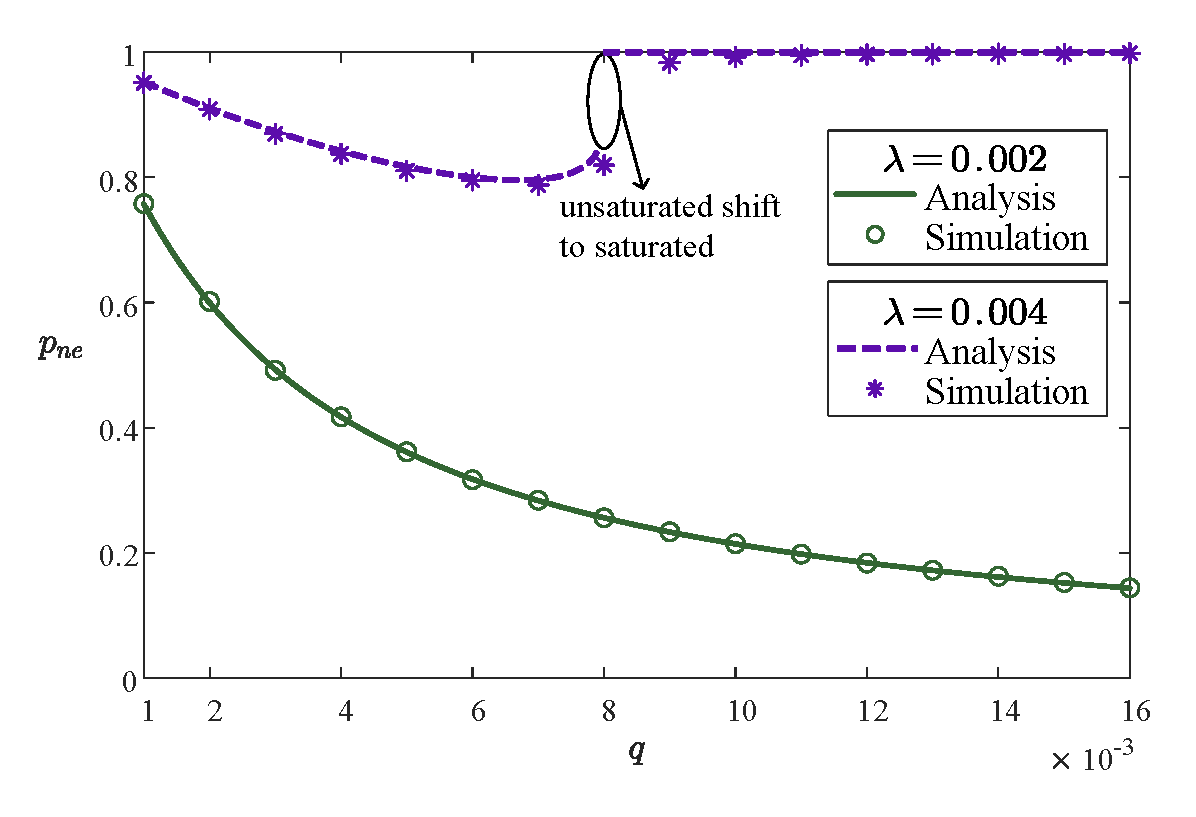
\includegraphics[width=\linewidth]{figure/chap3/p_ne_vs_q.pdf}
		\caption{节点缓存非空概率$p_{ne}$}
		\label{fig:p_ne}
	\end{subfigure}
	\hfill
	\begin{subfigure}{0.485\textwidth}
		\centering
		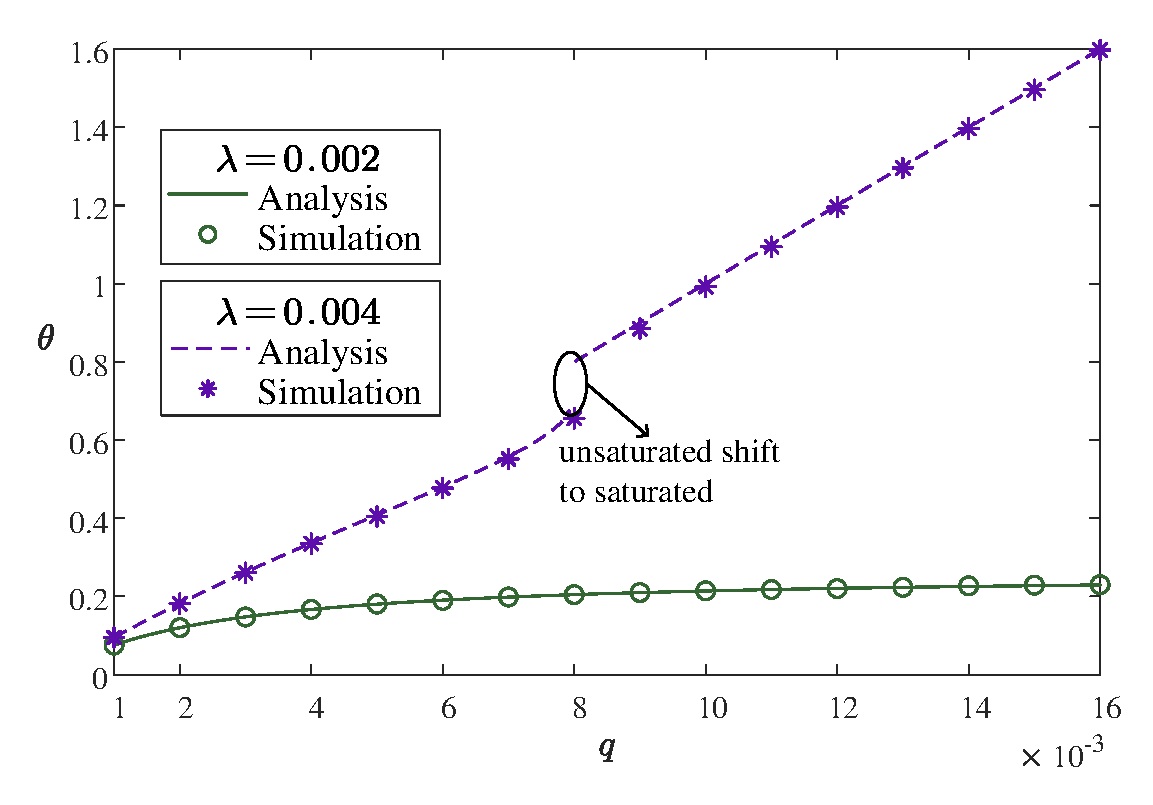
\includegraphics[width=\linewidth]{figure/chap3/theta_vs_q.pdf}
		\caption{尝试速率$\theta$}
		\label{fig:theta}
	\end{subfigure}
	
	\begin{subfigure}{0.495\textwidth}
		\centering
		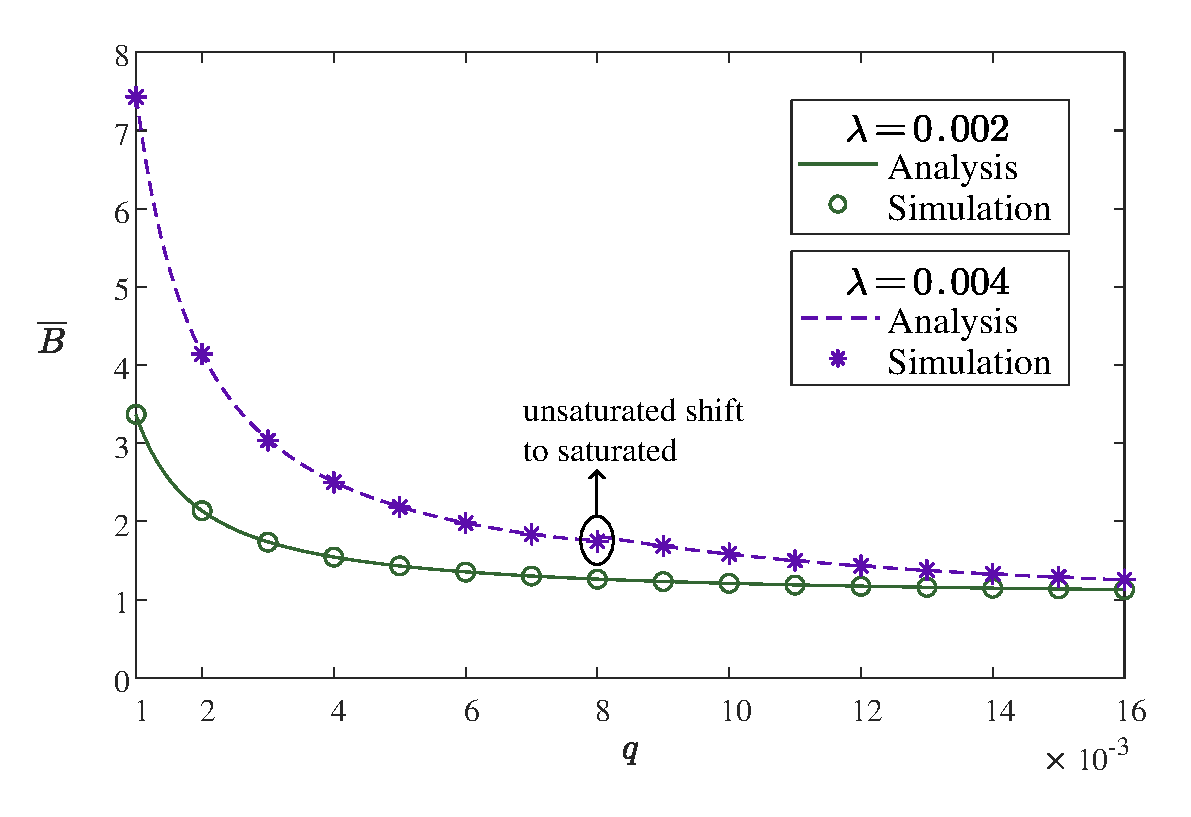
\includegraphics[width=\linewidth]{figure/chap3/mean_B_vs_q.pdf}
		\caption{信道忙期平均长度$\overline{B}$}
		\label{fig:mean_B}
	\end{subfigure}
	\hfill
	\begin{subfigure}{0.485\textwidth}
		\centering
		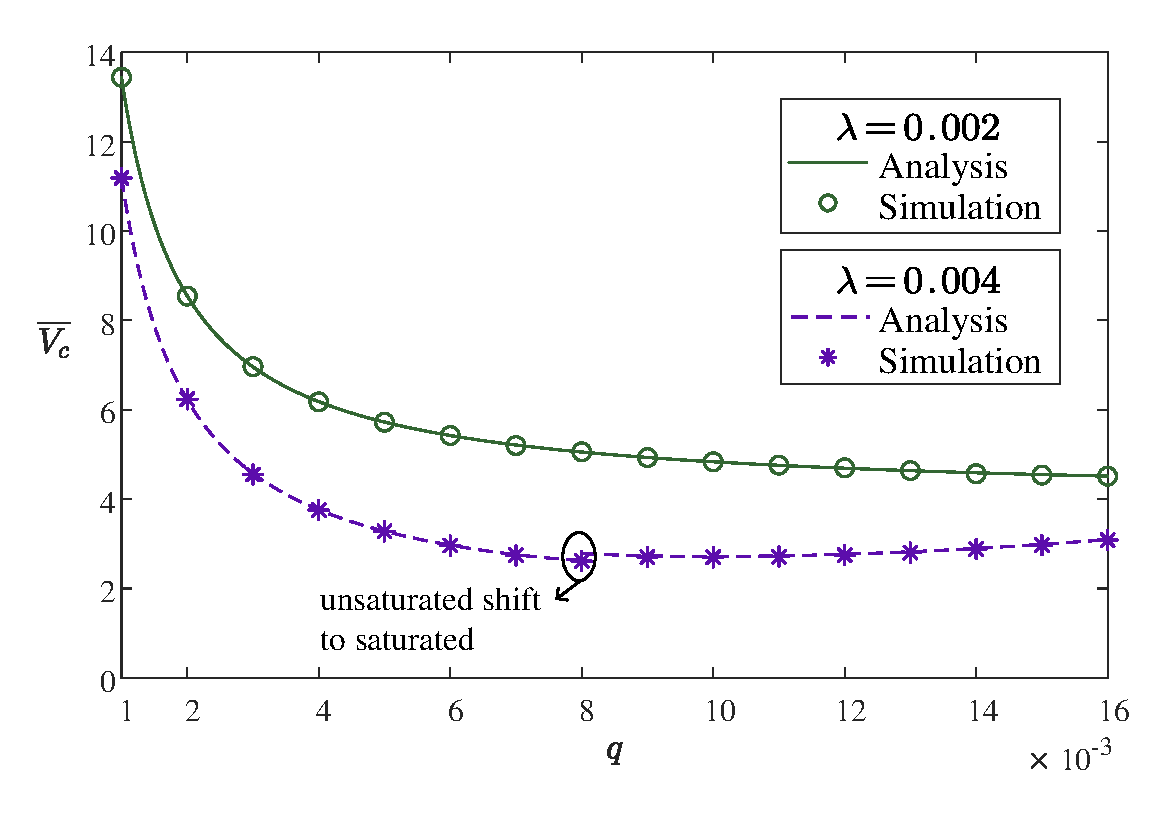
\includegraphics[width=\linewidth]{figure/chap3/mean_Vc_vs_q.pdf}
		\caption{信道假期平均长度$\overline{V}_c$}
		\label{fig:mean_Vc}
	\end{subfigure}
	\caption{系统参数随传输概率$q$的变化情况，$n=100$，$\lambda = \hat{\lambda}/n \in \{0.002, 0.004\}$}
	\label{fig:system_parameters}
\end{figure}

图 \ref{fig:p_ne} 至图 \ref{fig:mean_Vc} 展示了系统关键参数随传输概率 $q$ 的变化趋势。根据节点输入速率的不同，网络表现出两种截然不同的行为模式。首先，在轻负载条件下，例如 $\lambda=0.002$，网络始终处于非饱和稳态。随着传输概率 $q$ 的增加，尝试速率 $\theta$ 随之上升，表明接入竞争更加频繁。然而，由于信道资源尚有富余，较高的发送概率加速了数据包传输，使得节点能够更快地清空缓存。因此，节点缓存非空概率 $p_{ne}$、平均忙期 $\overline{B}$ 以及平均信道假期 $\overline{V}_c$ 均呈现单调递减趋势。
相比之下，在重负载条件下，例如 $\lambda=0.004$，系统行为出现明显差异。如图 \ref{fig:theta} 所示，随着 $q$ 的增加，曲线出现了一个明显转折点，标志着网络从非饱和状态向饱和状态转变。
其原因在于，当 $q$ 过大时，剧烈的信道竞争导致碰撞率飙升，系统的有效吞吐量开始低于数据包的到达速率。这导致数据包在节点缓存中迅速积压，使得节点缓存非空概率 $p_{ne}$ 迅速攀升并锁定在 1，网络随即陷入饱和。
在此饱和区域内，系统的尝试速率不再满足非饱和定点方程（式 \ref{eq:theta_fixed_point}），而是转由饱和条件下的线性关系 $\theta_{sa} = nq$ 主导。此外，图 \ref{fig:mean_B} 和图 \ref{fig:mean_Vc} 分别记录了该相变过程对平均忙期 $\overline{B}$ 和平均假期 $\overline{V}_c$ 的影响。可以观察到，尽管网络状态发生了根本性切换，这两个指标在饱和区的数值变化幅度相对平缓。



\section{吞吐量性能分析}
\label{sec:throughput_analysis}

本节基于前文休假排队模型分析 SAST机制下的吞吐量。为了探究 SAST 机制的性能极限，我们考虑网络处于饱和状态这一场景。在这一场景中，节点缓存始终非空（$p_{ne}=1$）、缓存清空概率为零（$p_0=0$），因此尝试速率为 $\theta_{sa}=nq$。将上述条件代入式 (\ref{eq:mean_vc_derived}) 与 $\overline{B}_{sa}$ 的表达式，可得饱和状态下的平均周期参数分别为	$ \overline{V}_{c,sa} = \frac{e^{nq}}{nq}, \quad \overline{B}_{sa} = \frac{1}{1 - e^{-nq}} $。
在将该结果代入吞吐量定义式，可得吞吐量的表达式为：
\begin{equation}
	\label{eq:access_throughput_sa}
	\lambda_{out}^a = \frac{nq (1 - e^{-nq})}{nq + e^{nq} - 1},
\end{equation}

\begin{equation}
	\label{eq:data_throughput_sa}
	\lambda_{out}^d = \frac{nq}{nq + e^{nq} - 1}.
\end{equation}
基于上述闭式解，我们可以通过调节传输概率 $q$ 来优化系统性能。以下两个定理分别给出了接入吞吐量和数据吞吐量的理论极限。
\begin{theorem}[最大接入吞吐量]
	\label{thm:max_access_throughput}
	当网络处于饱和状态时，SAST 机制的最大接入吞吐量约为 0.2384。该最大值当且仅当传输概率 $q$ 满足特定最优条件时取得：
	\begin{equation}
		\max_{q} \lambda_{out}^a \approx 0.2384, \quad \text{条件：} q^* \approx \frac{1.2515}{n}.
	\end{equation}
\end{theorem}

\begin{proof}
	令 $x = nq$，构造函数 $f(x) = \lambda_{out}^a(x)$。对 $f(x)$ 求导并令 $f'(x) = 0$，可得关于 $x$ 的超越方程。通过数值方法求解该方程，可得极值点位于 $x_0 \approx 1.2515$ 处，对应的函数极大值为 $f(x_0) \approx 0.2384$。
%	详细的导数推导及数值求解过程参见\textbf{附录 D}。
\end{proof}
\begin{theorem}[最大数据吞吐量]
	\label{thm:max_data_throughput}
	当网络处于饱和状态时，数据吞吐量 $\lambda_{out}^d$ 是关于总负载 $nq$ 的单调递减函数。SAST 机制的理论最大数据吞吐量为 0.5，且在传输概率趋近于 0 时取得：
	\begin{equation}
		\lambda_{max}^d = \lim_{nq \to 0} \lambda_{out}^d = \frac{1}{2}.
	\end{equation}
\end{theorem}

\begin{proof}
	令 $x = nq$，构造函数 $g(x) = \lambda_{out}^d(x) = \frac{x}{x + e^x - 1}$。对 $g(x)$ 求导，可证在 $x > 0$ 的区间内 $g'(x) < 0$ 恒成立，即数据吞吐量随负载增加而单调递减。
	为了求取最大值，利用洛必达法则对 $x \to 0$ 处求极限：
	\[
	\lim_{x \to 0} \frac{x}{x + e^x - 1} = \lim_{x \to 0} \frac{1}{1 + e^x} = \frac{1}{2}.
	\]
%	详细的单调性证明过程参见\textbf{附录 D}。
\end{proof}
%定理 \ref{thm:max_data_throughput} 揭示了 SAST 机制的核心优势：通过降低传输概率 $q$（即 $nq \to 0$），虽然成功接入的频次降低，但单次接入后的平均忙期长度 $\overline{B}_{sa}$ 显著增加，从而能够极其高效地填充信道，突破了传统 Aloha 协议 $e^{-1} \approx 0.368$ 的性能瓶颈。
\begin{figure}[t]
	\centering
	% --- 子图 (a): 接入吞吐量 ---
	\begin{subfigure}[b]{0.495\textwidth}
		\centering
		% 请替换为您实际的图片文件名
		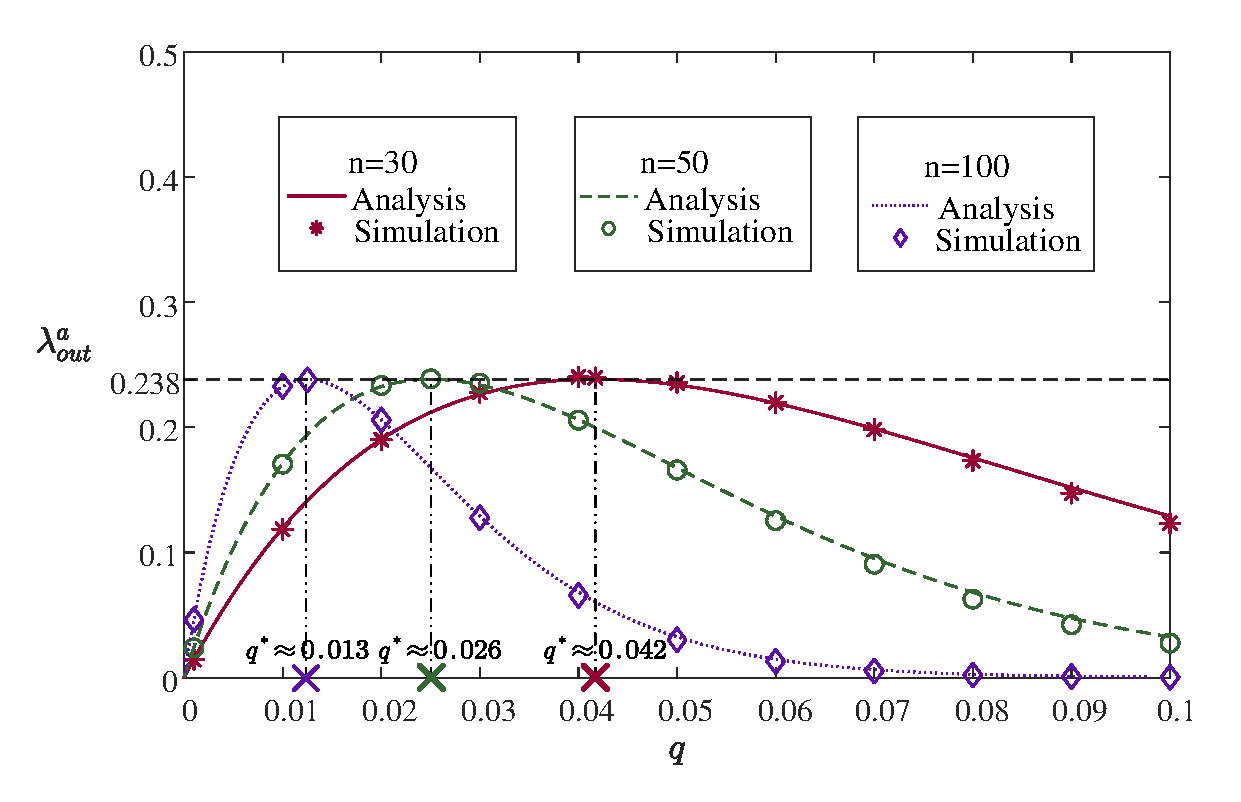
\includegraphics[width=\textwidth]{figure/chap3/access_throughput_vs_q.pdf}
		\caption{接入吞吐量 $\lambda_{out}^a$}
		\label{fig:sub_access}
	\end{subfigure}
	\hfill % 在两个子图之间添加弹性间距
	% --- 子图 (b): 数据吞吐量 ---
	\begin{subfigure}[b]{0.495\textwidth}
		\centering
		% 请替换为您实际的图片文件名
		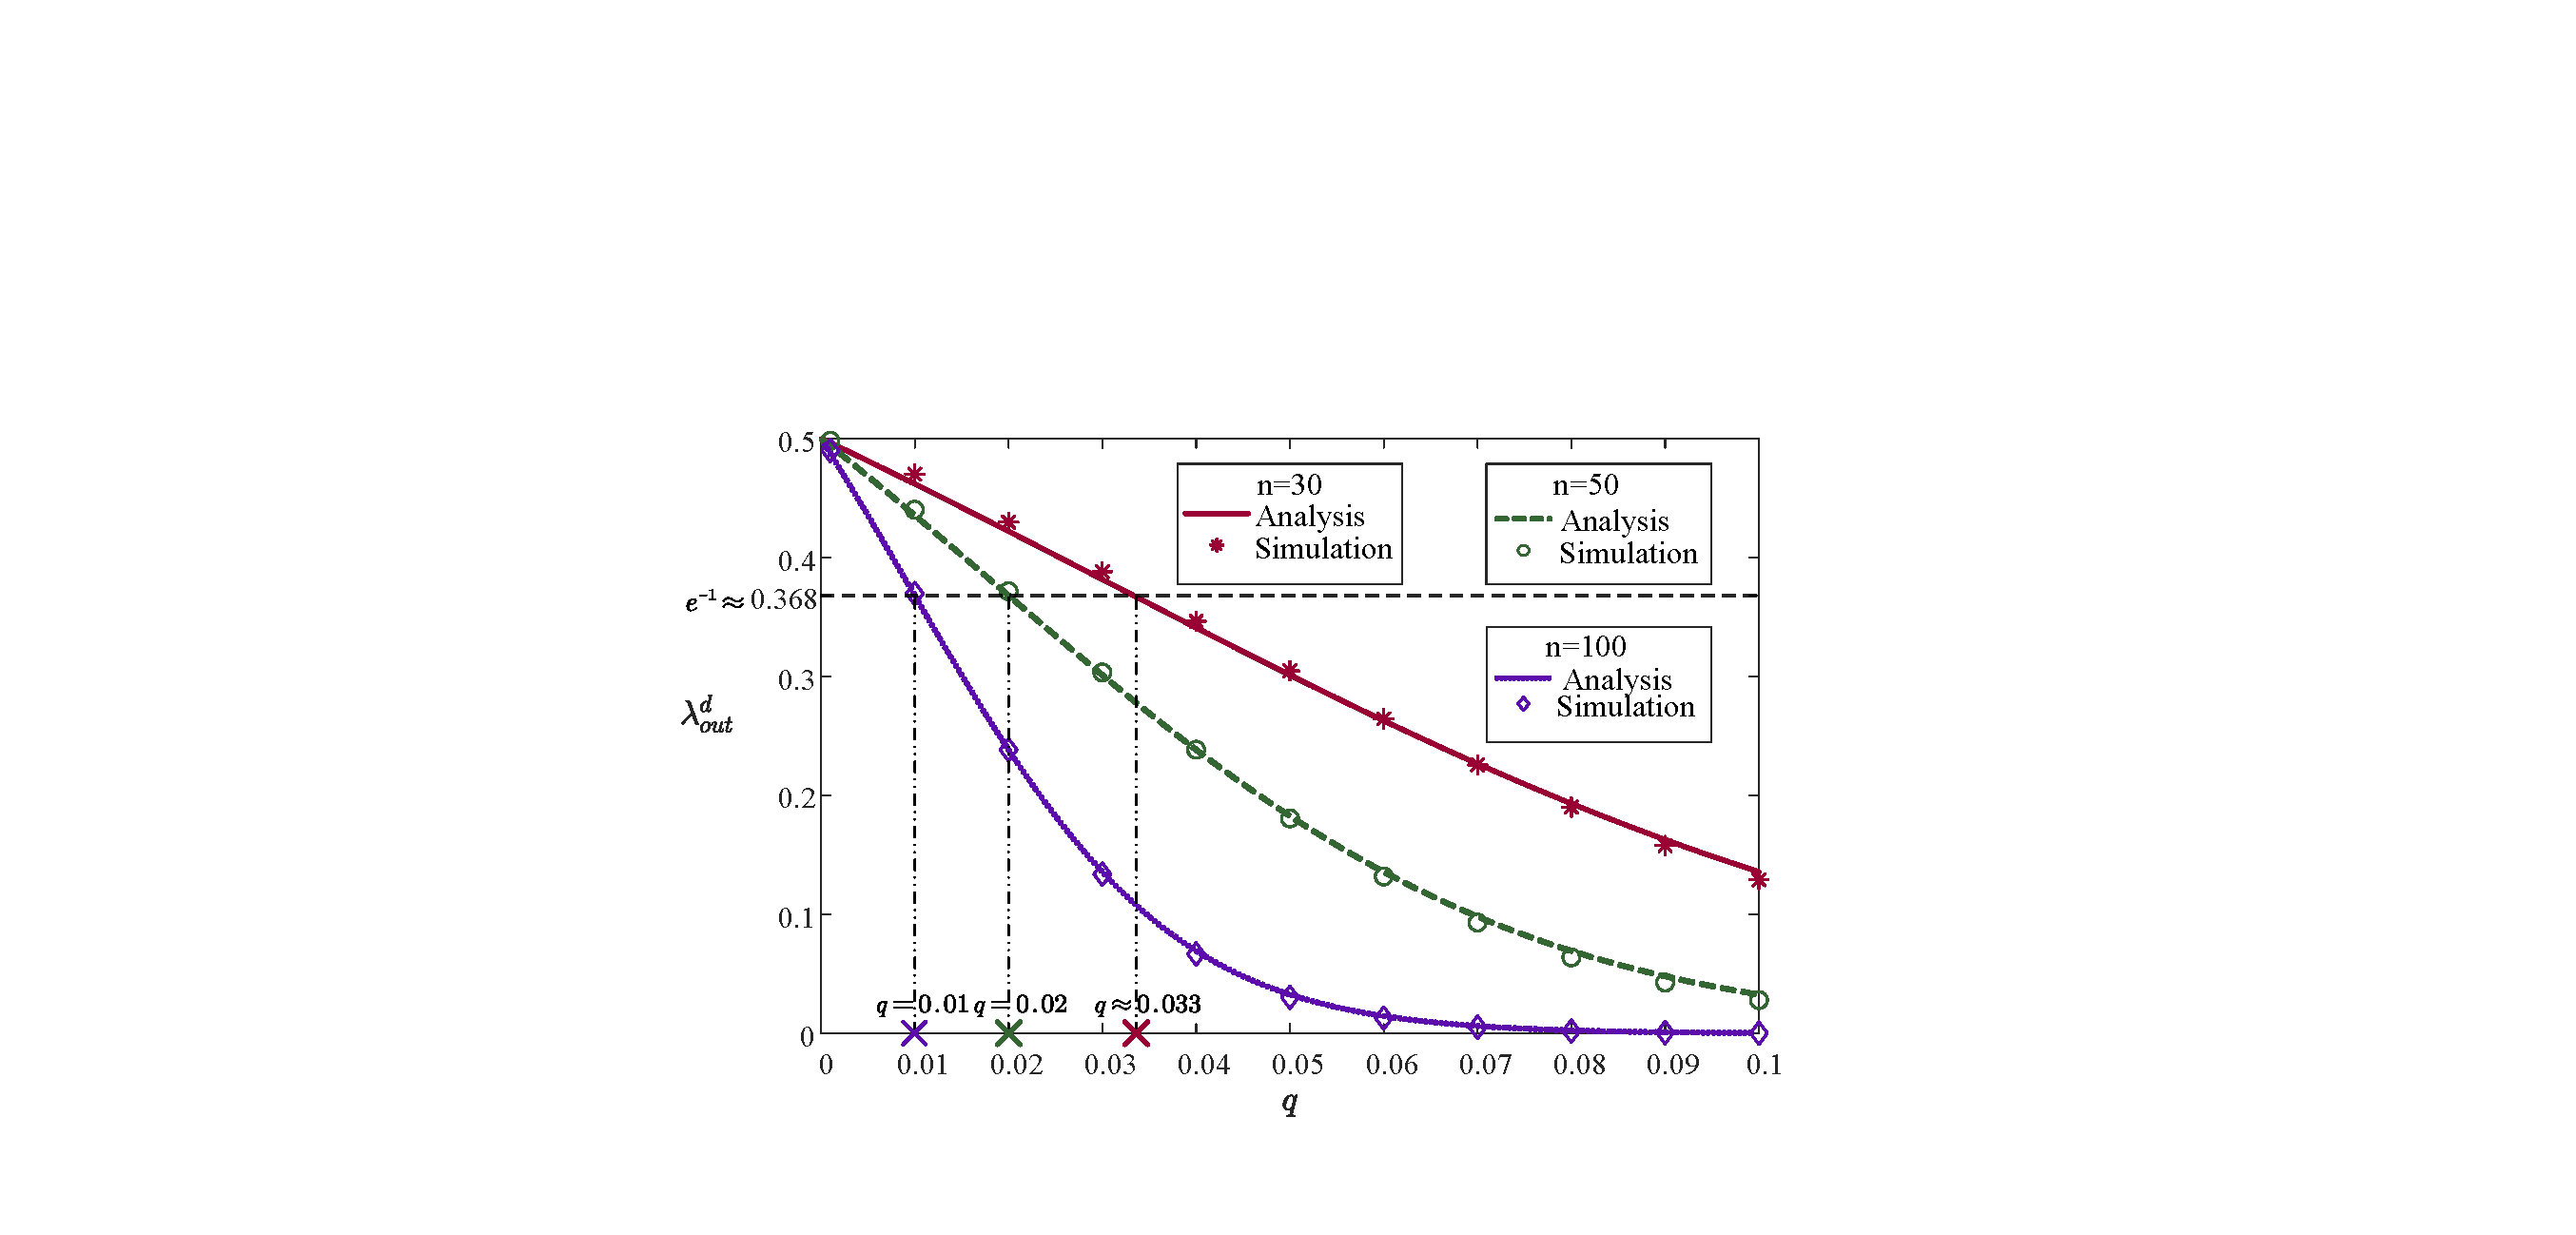
\includegraphics[width=\textwidth]{figure/chap3/data_throughput_vs_q.pdf}
		\caption{数据吞吐量 $\lambda_{out}^d$}
		\label{fig:sub_data}
	\end{subfigure}
	
	\caption{饱和状态下的吞吐量性能随传输概率 $q$ 的变化，$n \in \{30, 50, 100\}$}
	\label{fig:throughput_vs_q}
\end{figure}


为了验证上述理论推导的准确性，图 \ref{fig:throughput_vs_q} 展示了在饱和状态下，接入吞吐量 $\lambda_{out}^a$ 和数据吞吐量 $\lambda_{out}^d$ 随传输概率 $q$ 的变化情况。仿真中设置节点数量 $n \in \{30, 50, 100\}$。
如图~\ref{fig:sub_access} 所示，接入吞吐量随接入概率 $q$ 呈现出典型的先增后减的凸函数特征。在较小的 $q$ 区域内，节点发起接入的概率较低，系统整体处于轻载状态，此时信道竞争较弱，多数时隙处于空闲或仅有少量节点参与竞争的状态，虽然单次接入成功概率较高，但由于单位时间内的接入尝试次数有限，成功接入事件的总体数量受到限制，从而使接入吞吐量维持在较低水平。随着 $q$ 的逐步增大，参与竞争的节点数量增加，系统中的接入尝试频率提升，在碰撞尚未成为主导因素之前，成功接入事件的发生频率随之增加，从而推动接入吞吐量不断上升。当 $q$ 进一步接近最优点 $q^*$ 时，系统达到接入尝试频率与碰撞概率之间的平衡状态，此时单位时隙内平均参与竞争的节点数量处于一个最优水平，使得接入吞吐量达到峰值。随着 $q$ 超过该临界值，系统逐渐进入高竞争区域，大量节点在同一时隙内同时发起接入请求，导致碰撞概率迅速上升，而随机接入成功要求恰有一个节点发送，因此多节点同时发送会使成功概率呈指数形式下降，尽管接入尝试频率仍在增加，但绝大多数尝试由于碰撞而失效，信道被大量无效竞争占用，最终导致接入吞吐量快速下降。此外也可以观察到，其最优接入概率 $q^*$ 也不是 $\frac{1}{n}$，而是 $\frac{1.2515}{n}$；其根本原因在于连续传输机制导致最优点发生了偏移。



另一方面，图~\ref{fig:sub_data} 展示了数据吞吐量随接入概率 $q$ 的变化规律。可以观察到，随着 $q$ 的增大，数据吞吐量整体呈现单调递减趋势。以经典时隙 Aloha 的最大吞吐量 $e^{-1} \approx 0.368$ 作为基准线，当系统总负载满足 $nq < 1$ 时，SAST 机制的数据吞吐量始终高于该基准，并可接近 0.5。这一现象源于接入频率与碰撞概率之间的权衡关系，即较小的 $q$ 虽然降低了节点发起接入的频率，但同时抑制了多节点同时发送所引发的碰撞概率，从而使节点一旦成功接入信道，能够维持较长的连续传输过程，使平均忙期长度 $\overline{B}$ 增加，并通过更长时间的信道占用来承载更多数据传输。
随着 $q$ 的增大，系统竞争强度逐渐增强，碰撞概率上升，不仅降低了接入成功概率，更会频繁打断已经建立的连续传输过程，从而导致忙期长度缩短。尽管更大的 $q$ 在一定程度上有利于增加成功接入事件的发生次数，但由于连续传输阶段被频繁打断，使单次成功接入所能传输的数据包数量减少，且这种下降速度快于接入频率提升所带来的收益增长，因此系统整体吞吐量呈现出持续下降的趋势。
特别地，这一单调下降特性与经典时隙 Aloha 中的凸性规律本质不同，其根本原因在于系统吞吐量的主导因素发生了转变。系统性能主要由单位时隙内的成功接入概率决定，因此在较小的 $q$ 区域内，随着节点发送概率的提高，成功发送事件的发生频率增加，从而带来吞吐量的提升；而当 $q$ 进一步增大时，多用户竞争导致的碰撞概率迅速上升并逐渐占据主导地位，最终使吞吐量下降，形成典型的凸形变化趋势。然而在 SAST 机制中，数据吞吐量不仅取决于接入成功的发生频率，还与单次成功接入后所能维持的连续传输时长，即忙期长度$\overline{B}$ 密切相关，系统整体性能可以理解为接入成功过程与连续占用信道过程的共同结果。



\section{时延性能分析}
\label{sec:delay_analysis}
除了吞吐量之外，时延是衡量随机接入机制性能的另一项关键指标。本节将分别对接入时延 $D_A$ 和数据包时延 $D_P$ 进行推导。

\subsection{接入时延 $D_A$ 推导与分析}

接入时延 $D_A$ 定义为节点生成的队首数据包从进入队首开始，到成功被基站接收并收到确认反馈为止所经历的平均时长。
从前文节点休假模型可知，接入过程本质上对应于类型 1 假期，即节点在缓存非空的情况下不断竞争信道直至成功的时段。因此，接入时延在数值上等同于类型 1 假期的平均长度：
\begin{equation}
	D_A = \overline{V}_1.
\end{equation}

结合前文关于类型 1 假期的新包到达过程 $A_{V_1}$ 的推导以及节点输入的伯努利特性，根据排队论中的 Little 定律，可得 $D_A = \overline{V}_1 = \frac{\overline{A}_{V_1}}{\lambda}$。
将前文推导的 $\overline{A}_{V_1}$ 闭式解代入，可得非饱和情况下，接入时延的通用表达式：
\begin{equation}
	\label{eq:access_delay_general}
	D_A = \frac{\theta}{n q \lambda \left(1 - \frac{\theta}{n q} e^{-\theta}\right)}.
\end{equation}

特别地，当网络处于饱和状态时，我们从单节点的接入吞吐量与其平均接入时延之间的关系出发。注意，此时节点的所有假期都为类型1假期。
单节点的接入吞吐量可以表示为 $\lambda_{out}^a / n = \frac{1}{\overline{ B }+ \overline{V_{1,sa}}}= \frac{q(1 - e^{-nq})}{nq+e^{nq}-1}$。由此可得饱和状态下的平均接入时延为
\begin{equation}
	\label{eq:access_delay_sa}
	D_{A,sa} = \overline{V}_{1,sa} = \frac{e^{nq} + nq - 1 - q}{q(1 - e^{-nq})}.
\end{equation}
该式表明，在饱和状态下，接入时延主要受总负载 $nq$ 的指数增长项主导。


\subsection{数据包时延 $D_P$ 推导与分析}
数据包时延 $D_P$ 定义为数据包从生成时刻起到成功传输完毕离开系统所需的平均时长，该指标由排队等待时间和传输服务时间两部分组成。
需要说明的是，数据包时延的稳态分析仅在网络处于非饱和状态，即数据吞吐量等于输入速率 $\lambda_{out}^d = n\lambda$ 时有效。若网络处于饱和状态，节点缓存队列长度发散，导致理论上的平均包时延趋于无穷大。

为了求解 $D_P$，我们借助排队论中的 Little 定律 $D_P = \frac{\overline{L}}{\lambda}$，其中 $\overline{L}$ 为节点缓存队列的平均长度。因此，问题的核心转化为求解稳态下的平均队长 $\overline{L}$。
为此，我们引入一个二维马尔可夫链 $(L_t, K_t)$ 来刻画节点队列的动态行为，如图 \ref{fig:markov_chain} 所示。其中，$L_t \in \{0, 1, \dots\}$ 表示时隙 $t$ 开始时的队列长度，$K_t \in \{0, 1\}$ 为状态指示变量，$K_t=1$ 表示节点处于忙期，$K_t=0$ 表示节点处于假期。

\begin{figure}[t]
	\centering
	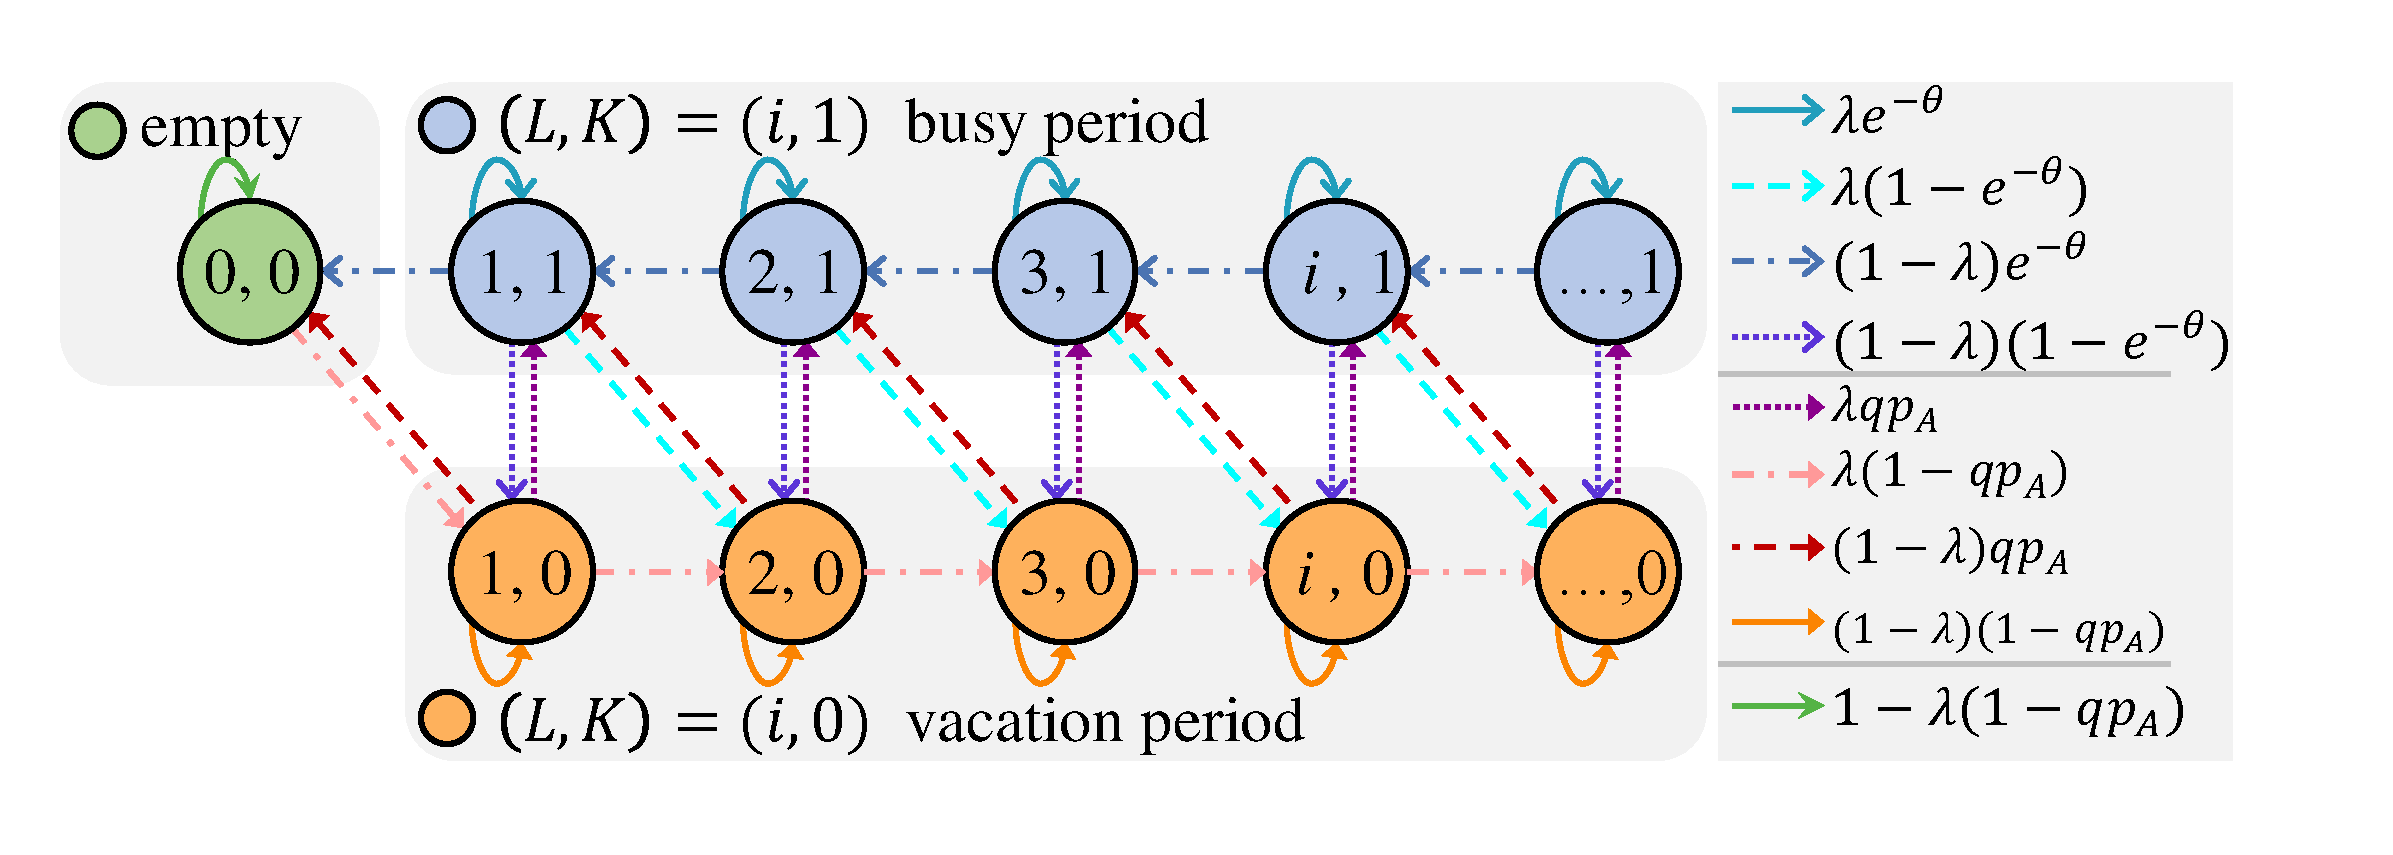
\includegraphics[width=0.95\textwidth]{figure/chap3/2Dmarkov_chain.pdf}
	\caption{节点队列长度在时隙 $t$ 的状态转移马尔可夫链 $(L_t, K_t)$}
	\label{fig:markov_chain}
\end{figure}
通过求解该马尔可夫链的平衡方程，可得其稳态概率分布 $\pi_{i,k} = \lim_{t\to\infty} \Pr\{L_t=i, K_t=k\}$ 如下：
\begin{equation}
	\label{eq:steady_state_prob}
	\begin{cases}
		\pi_{10} = \left( \dfrac{1}{1 - \frac{\lambda}{1-\lambda}\gamma} + \dfrac{\lambda}{1-\lambda} - 1 + \dfrac{1}{1-\gamma} + \dfrac{(1-\lambda)p_A + \lambda e^{-\theta}}{\lambda(1-p_A)} \right)^{-1} \\
		\pi_{00} = \dfrac{(1-\lambda)p_A + \lambda e^{-\theta}}{\lambda(1-p_A)} \pi_{10} \\
		\pi_{11} = \dfrac{\lambda}{1-\lambda} \pi_{10} \\
		\pi_{i0} = \gamma^{i-1} \pi_{10}, \quad i \geq 2 \\
		\pi_{i1} = \dfrac{\lambda}{1-\lambda} \pi_{i0} = \left( \dfrac{\lambda}{1-\lambda} \gamma \right)^{i-1} \pi_{10}, \quad i \geq 2
	\end{cases}
\end{equation}
式中，参数 $\gamma$ 定义为
$ 	\gamma = \frac{\lambda[\lambda(1-e^{-\theta}) + (1-\lambda)(1-p_A)]}{(1-\lambda)(\lambda e^{-\theta} + (1-\lambda)p_A)}$。 $p_A$ 定义为接入请求概率。
基于稳态分布，节点缓存队列的平均长度可由期望公式计算得出：$\overline{L} = \mathbb{E}[\pi] = \sum_{i=1}^{\infty} (\pi_{i0} + \pi_{i1}) i$。

在 SAST 机制中，队首数据包成功接入的前提是信道处于可用状态且其余节点未同时竞争。信道可用包含两种互斥情况：一是信道处于休假状态，其概率为 $1 - \lambda_{out}^{d}$；二是信道处于忙期的最后一个时隙，且当前传输节点在该忙期结束时恰好清空缓存。后一事件在每个信道周期中至多出现一次，因此对应概率可写为 $p_0 / \overline{C}_c$。进一步结合其余 $n-1$ 个节点的静默概率 $e^{-\theta}$，可得接入成功概率 $p_A$ 为：
\begin{equation}
	\label{eq:pA_expression}
	p_A = \left(1 - \frac{\lambda \theta}{q}\right) e^{-\theta}
\end{equation}
将 $p_A$ 代入稳态分布并求和，得到节点缓存队列平均长度 $\overline{L}$ 的闭式解：
\begin{equation}
	\label{eq:mean_queue_length}
	\overline{L} = \frac{ \frac{1}{1-\lambda} + \frac{\gamma(2-\gamma)}{(1-\gamma)^2} + \frac{\frac{\lambda\gamma}{1-\lambda} \left(2 - \frac{\lambda\gamma}{1-\lambda}\right)}{\left(1 - \frac{\lambda\gamma}{1-\lambda}\right)^2} }{ \frac{1}{1 - \frac{\lambda\gamma}{1-\lambda}} + \frac{\lambda}{1-\lambda} - 1 + \frac{1}{1-\lambda} + \frac{(1-\lambda)p_A + \lambda e^{-\theta}}{\lambda(1-p_A)} }.
\end{equation}
最终，将式 \eqref{eq:mean_queue_length} 除以输入速率 $\lambda$，即可得到非饱和状态下的平均数据包时延 $D_P$：
\begin{equation}
	\label{eq:mean_packet_delay}
	D_P = \frac{ \frac{1}{1-\lambda} + \frac{\gamma(2-\gamma)}{(1-\gamma)^2} + \frac{\frac{\lambda\gamma}{1-\lambda} \left(2 - \frac{\lambda\gamma}{1-\lambda}\right)}{\left(1 - \frac{\lambda\gamma}{1-\lambda}\right)^2} }
	{ \lambda ( \frac{1}{1 - \frac{\lambda\gamma}{1-\lambda}} + \frac{\lambda}{1-\lambda} - 1 + \frac{1}{1-\lambda} + \frac{(1-\lambda)p_A + \lambda e^{-\theta}}{\lambda(1-p_A)} )} .
\end{equation}
尽管式 \eqref{eq:mean_packet_delay} 形式较为复杂，但它建立了时延与系统参数（$n, q, \lambda$）之间的准确关系，为后续的时延性能优化提供了理论依据。
\begin{figure}[t]
	\centering
	\begin{subfigure}{0.495\textwidth}
		\centering
		% 请确保路径和文件名正确
		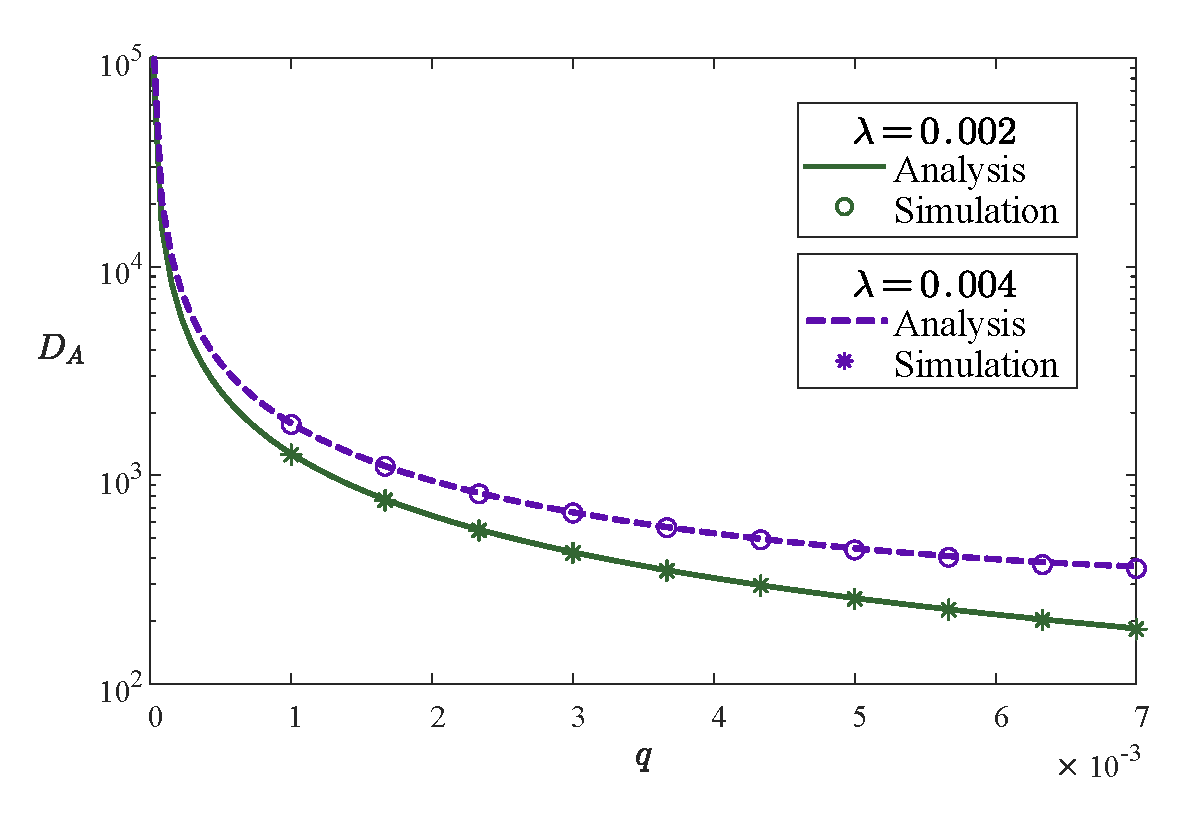
\includegraphics[width=\linewidth]{figure/chap3/access_delay_unsaturated.pdf}
		\caption{非饱和情况下平均接入时延 $D_A$}
		\label{fig:access_delay_unsaturated}
	\end{subfigure}
	\hfill
	\begin{subfigure}{0.495\textwidth}
		\centering
		% 请确保路径和文件名正确
		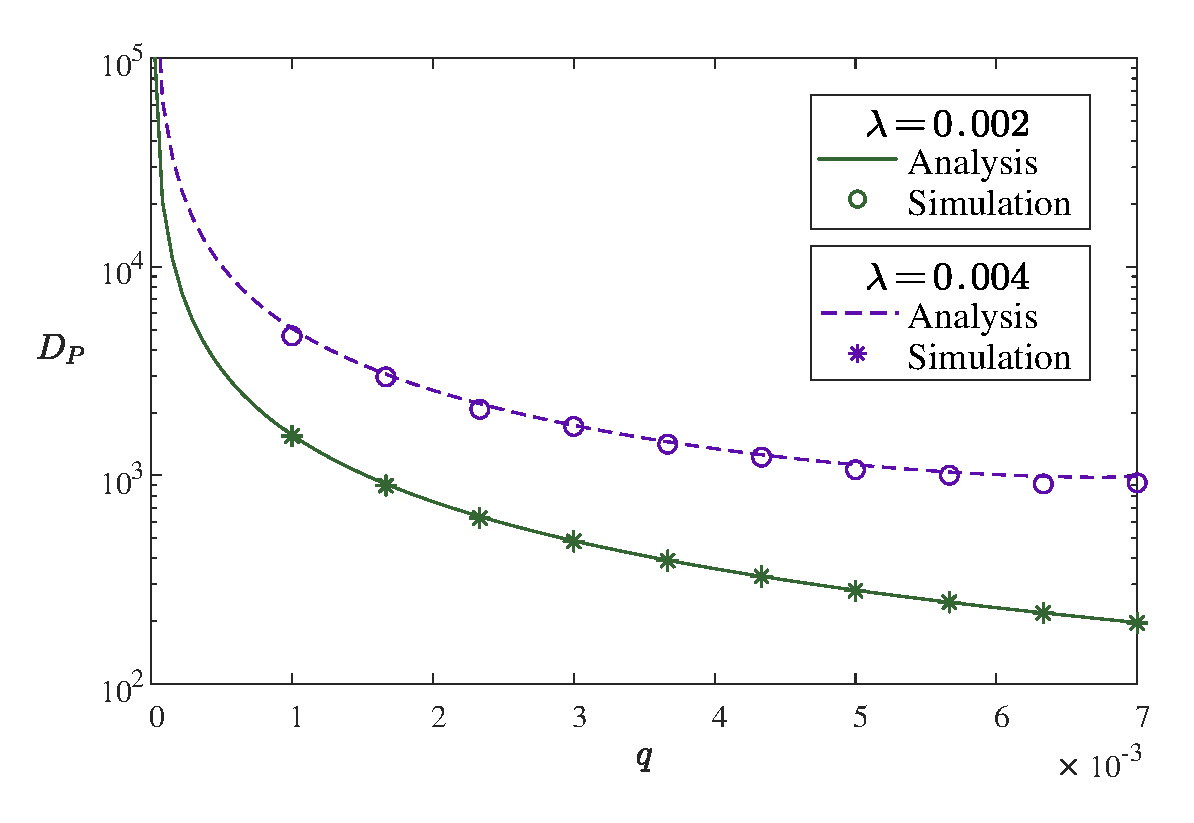
\includegraphics[width=\linewidth]{figure/chap3/packet_delay_unsaturated.pdf}
		\caption{非饱和情况下平均数据包时延 $D_P$}
		\label{fig:packet_delay_unsaturated}
	\end{subfigure}
	
	\begin{subfigure}{0.495\textwidth}
		\centering
		% 请确保路径和文件名正确
		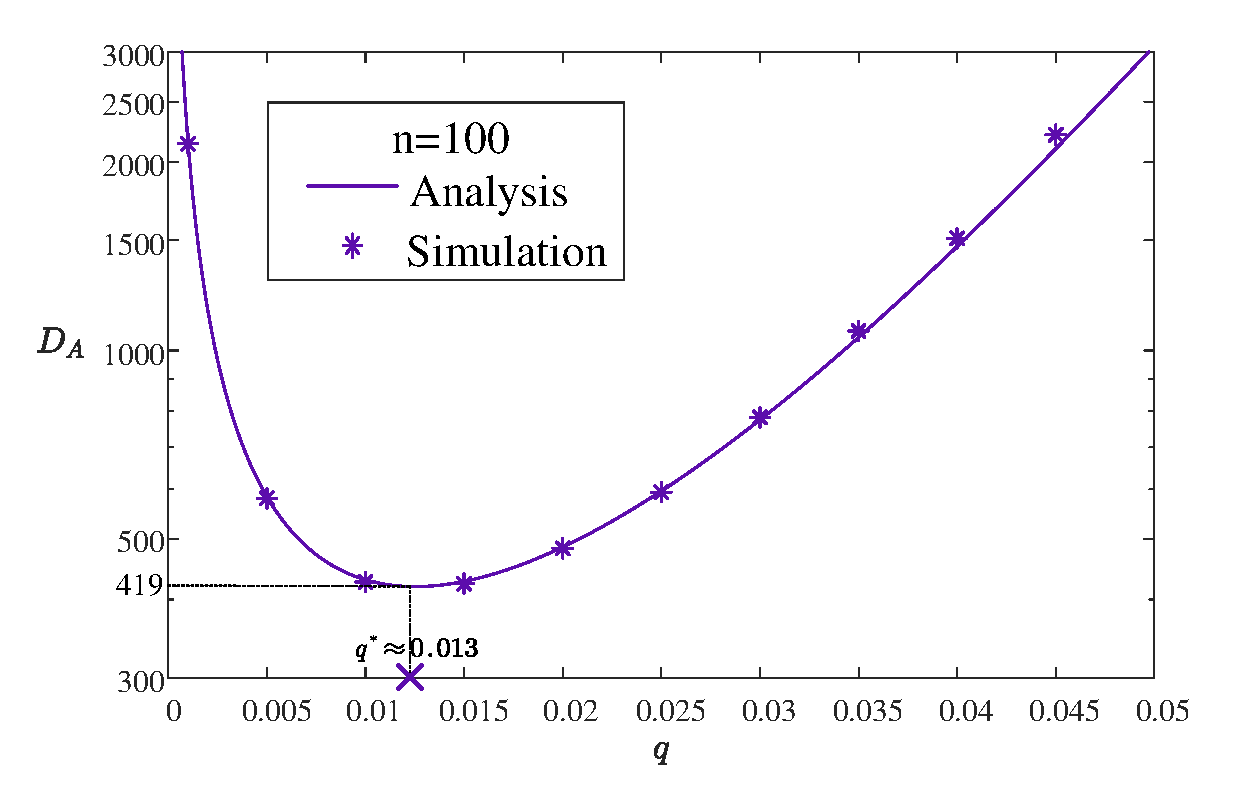
\includegraphics[width=\linewidth]{figure/chap3/access_delay_saturated.pdf}
		\caption{饱和情况下平均接入时延 $D_{A,sa}$}
		\label{fig:access_delay_saturated}
	\end{subfigure}
	\caption{时延随传输概率$q$的变化情况，$n=100$，$\lambda = \hat{\lambda}/n \in \{0.002, 0.004\}$}
	\label{fig:delay_vs_q}
\end{figure}


为了展示 SAST 机制的时延特性，图 \ref{fig:delay_vs_q} 给出了接入时延和数据包时延随传输概率 $q$ 的变化曲线。
如图 \ref{fig:access_delay_unsaturated} 和图 \ref{fig:packet_delay_unsaturated} 所示，当网络处于非饱和状态时，平均接入时延 $D_A$ 和平均包时延 $D_P$ 均随着传输概率 $q$ 的增加而单调递减。
这一现象的原因在于，在轻载（$\lambda=0.002$）或中载（$\lambda=0.004$）条件下，信道资源相对充裕，碰撞并非主要瓶颈。此时，增加 $q$ 使得节点在有数据包到达时能够更积极地尝试接入信道，从而减少了在队列头部的空闲等待时间，实现了数据包的快速发送。
图 \ref{fig:access_delay_saturated} 展示了饱和状态下接入时延 $D_{A,sa}$ 的变化趋势。与非饱和状态截然不同，$D_{A,sa}$ 随 $q$ 呈现出先减后增的凹函数特性。当 $q$ 较小时，增加传输概率有助于利用空闲信道，从而降低时延；当 $q$ 超过一定阈值，对应于最优负载点 $q^*$ 后，信道内的碰撞加剧。此时，节点频繁遭遇传输失败并退避，导致队首数据包滞留时间急剧增加。
对比前文的吞吐量分析可知，饱和接入时延取得最小值的点，恰好对应于接入吞吐量 $\lambda_{out}^a$ 取得最大值的点。这表明在饱和网络中，通过优化 $q$ 可以同时实现接入效率的最优和接入时延的最小化。


\section{SAST 机制在5G小数据传输中的性能评估}
\label{sec:5g_case_study}

\begin{figure}[t]
	\centering
	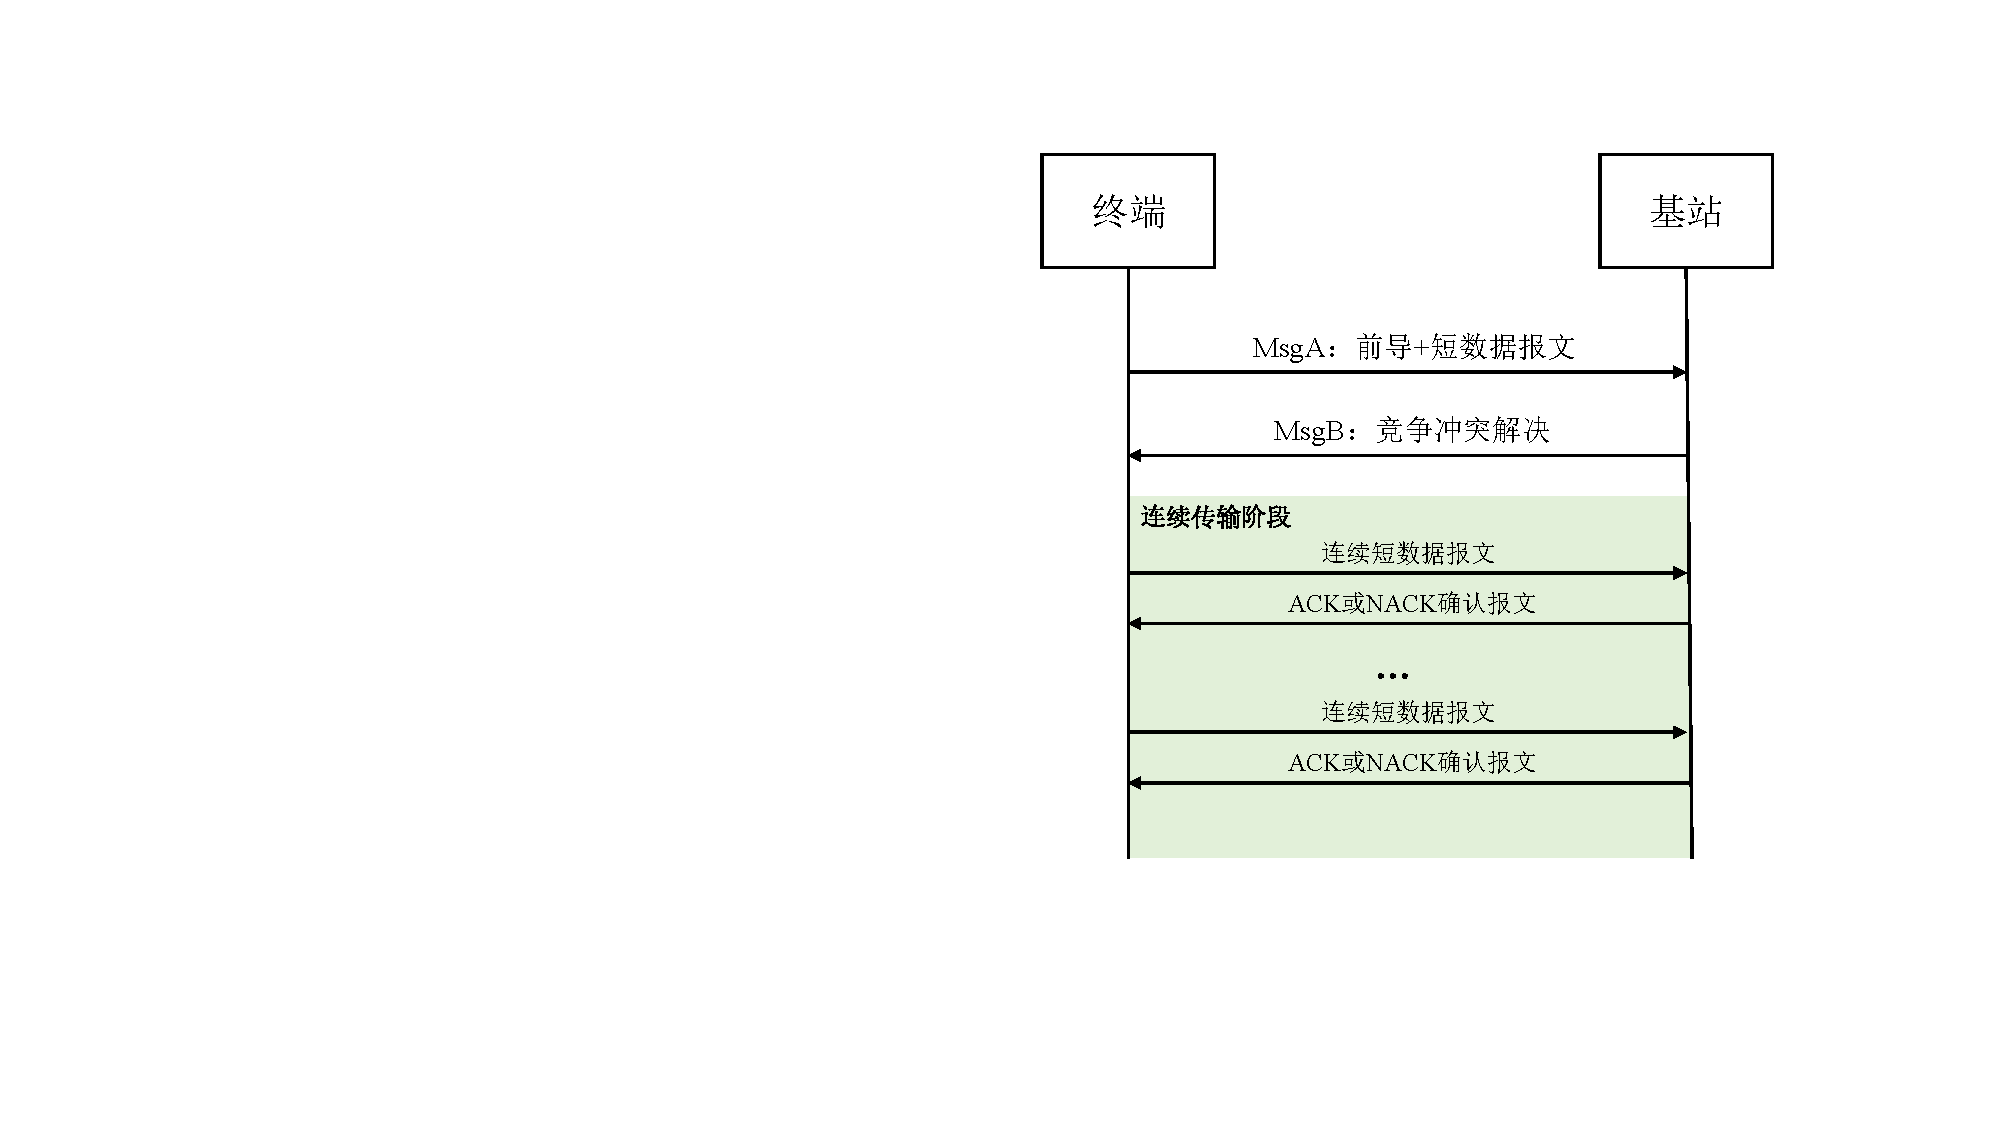
\includegraphics[width=0.65\textwidth]{figure/chap3/sast_scheme.pdf}
	\caption{SAST 方案下，用户与基站间的信令交互流程}
	\label{fig:signaling_process}
\end{figure}

	为了验证 SAST 机制在实际通信系统中的应用潜力，本节将其与 3GPP Release 17 标准中定义的 2 步小数据传输方案作为基准进行对比。为量化两者在控制信令开销方面的差异，本文引入信令吞吐比 $\mathrm{STR}$ 作为核心评估指标。

	\subsection{2 步小数据传输方案}

为克服传统蜂窝网络中 RRC 连接建立过程对小数据包传输造成的效率瓶颈，3GPP R17 标准引入了 2 步小数据传输方案。如图 \ref{fig:sdt_access} 中的 2 步小数据传输过程所示，该方案的核心机制是将物理随机接入信道前导码与上行共享信道的数据载荷合并封装于 MsgA 中发送。基站接收后回复包含竞争解决标识的 MsgB，以确认传输成功；若发生碰撞或解码失败，终端则需退避并重新发起 MsgA 传输。

从信令开销角度看，无论单次接入尝试是否成功，系统物理层都需要承担 MsgA 与 MsgB 两次信令交互的开销。设每次信令交互的平均大小为 $s$ 比特，若系统平均接入成功概率为 $p_A$，则成功传输一个数据包在统计上平均需要 $1/p_A$ 次尝试。据此，2 步小数据传输方案的信令吞吐比可表示为：
\begin{equation}
	\mathrm{STR}_{\mathrm{SDT}} = \frac{2s}{p_A}.
\end{equation}
其中，$p_A$ 可由文献\cite{2012_DaiAloha} 计算得到。这一指标直观地反映了在低接入成功率场景下，标准方案面临的信令效率急剧下降问题。

\subsection{SAST 机制在 5G 中的实现与信令分析}

SAST 机制在 5G 系统中的部署具有较强兼容性，可以复用 3GPP R17 的 2 步小数据传输流程完成初始接入，并在此基础上扩展连续传输能力以提升信令效率。
如图~\ref{fig:signaling_process} 所示，具体流程如下：节点首先将队首数据包封装在包含前导码的 MsgA 中发送，这与标准 2 步小数据传输过程一致。一旦收到基站反馈的 MsgB 并确认接入成功，节点随即进入连续传输阶段。与标准方案不同的是，后续数据包可直接在 PUSCH 信道发送，而无需再次携带前导码。基站对每个后续数据包逐一反馈确认消息；若成功传输一个报文，基站会回馈确认消息；若发生碰撞并收到否定确认消息，节点退回竞争状态。若节点缓存队列清空，则可通过最后一个数据报文中的结束标记告知基站传输即将结束，至此本轮传输自然结束。



为了量化上述机制带来的信令增益，下面分析其信令吞吐比 $\mathrm{STR}$。在 SAST 的一个成功接入周期内，平均可连续传输 $\overline{B}$ 个数据包。除队首数据包外，后续 $\overline{B}-1$ 个数据包的信令开销取决于忙期的结束方式：若传输因缓存清空而正常结束，概率为 $p_0$，则仅消耗对应的确认消息开销；若因碰撞而异常中断，概率为 $1-p_0$，则最后一个失败数据包还会额外消耗一次发送与一次否定确认的信令资源。
综合考虑队首数据包的初始接入与后续传输开销，SAST 的信令吞吐比可推导为：
\begin{equation}
	\mathrm{STR}_{\mathrm{SAST}} = s + \frac{s}{\overline{B}} \left( \frac{2}{p_A} + 1 - 2p_0 \right).
\end{equation}
特别地，在网络处于饱和极限状态下（此时 $p_0=0$ 且 $\theta=nq$），该指标可进一步简化为：
\begin{equation}
	\mathrm{STR}_{\mathrm{SAST}, sa} = s (2e^{nq} + 2nq - e^{-nq}).
\end{equation}
该式表明，在饱和状态下，SAST 通过一次前导码开销换取了多次数据传输机会，从而在理论上降低了单位数据的信令成本。

\subsection{信令开销性能对比}

\begin{figure}[t]
	\centering
	\begin{subfigure}[b]{0.48\textwidth}
		\centering
		% 对应 TCOM Fig. 8a
		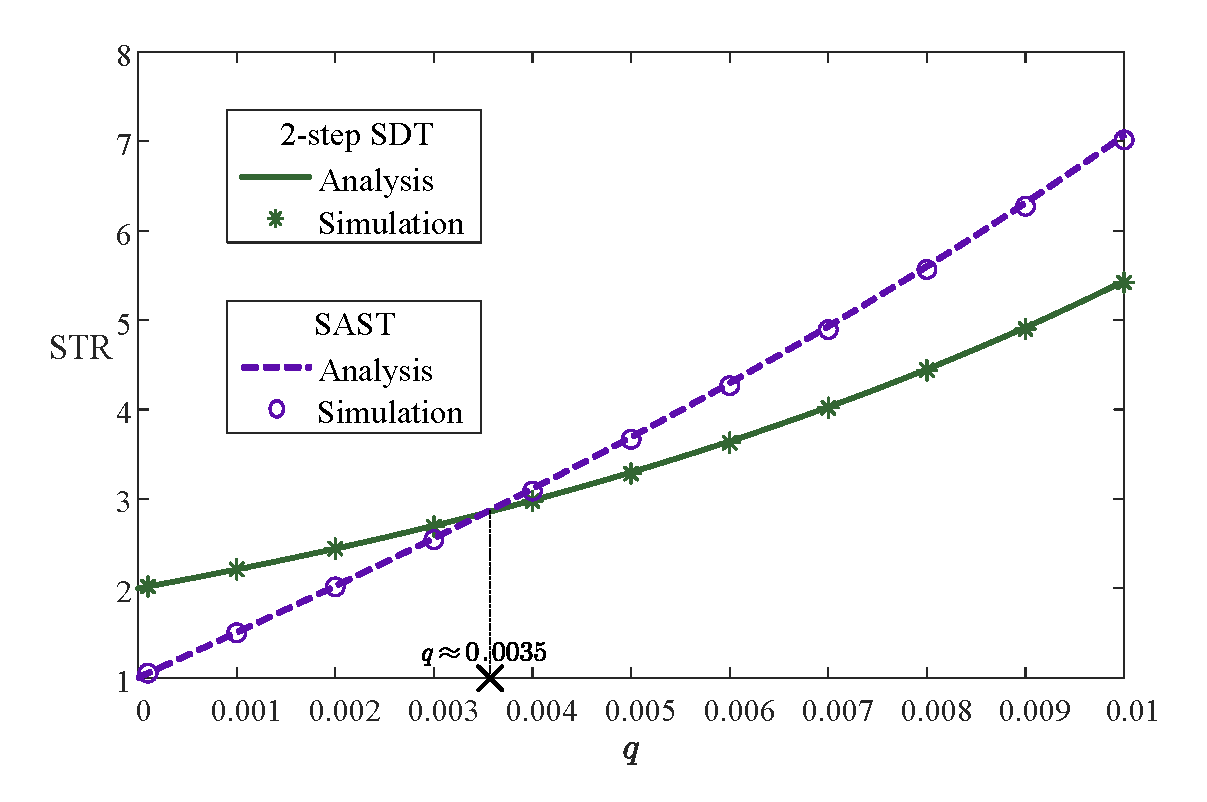
\includegraphics[width=\textwidth]{figure/chap3/str_vs_q_saturated.pdf}
		\caption{饱和状态下的 STR 对比}
		\label{fig:str_sat}
	\end{subfigure}
	\hfill
	\begin{subfigure}[b]{0.49\textwidth}
		\centering
		% 对应 TCOM Fig. 8b
		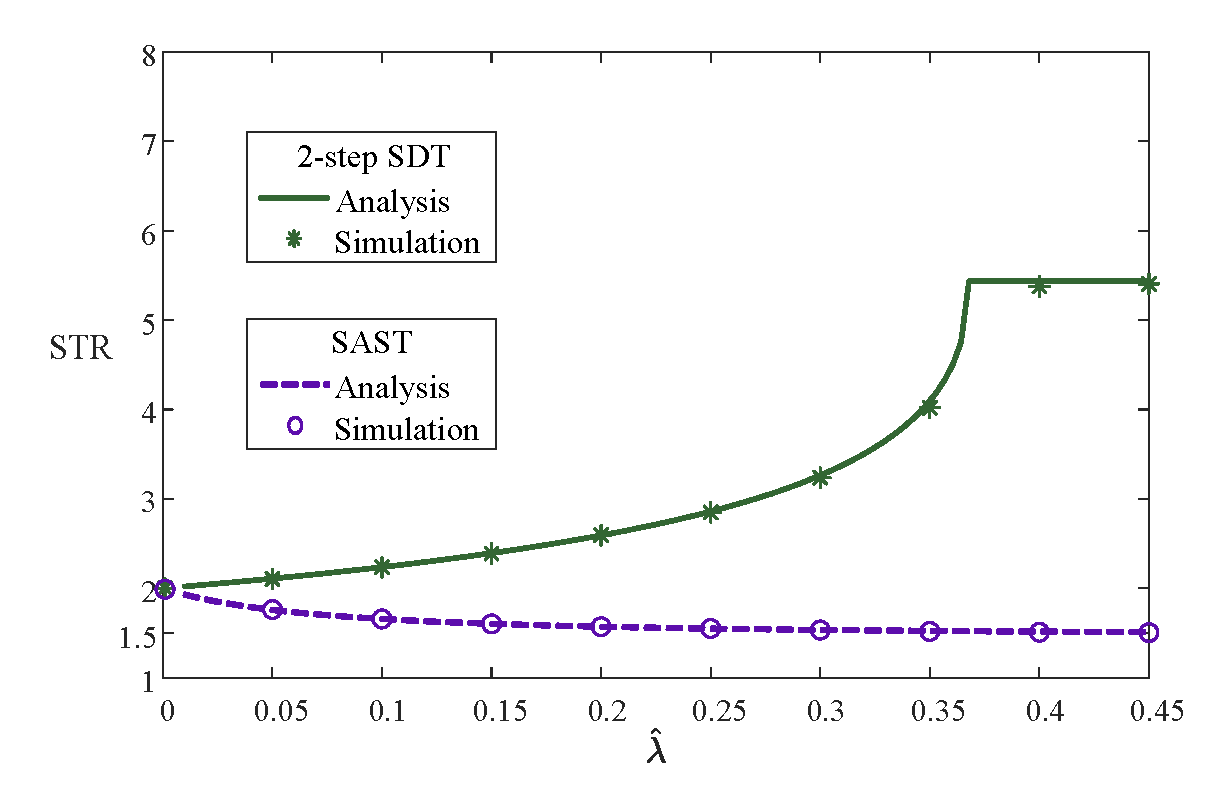
\includegraphics[width=\textwidth]{figure/chap3/str_vs_lambda_unsaturated.pdf}
		\caption{非饱和状态下的 STR 对比}
		\label{fig:str_unsat}
	\end{subfigure}
	\caption{SAST 与 2 步小数据传输方案的信令吞吐比性能对比，$n=100, s=1$}
	\label{fig:str_comparison}
\end{figure}

为直观展示两种方案性能差异，图 \ref{fig:str_comparison} 对比了不同负载条件下 STR 随传输概率 $q$ 的变化。
图~\ref{fig:str_sat} 给出了饱和状态下两种机制的信令吞吐比对比结果。在较小的接入概率 $q$ 区域内，SAST 方案的信令吞吐比明显低于 2 步小数据传输方案，其优势来源于信令分摊，即节点成功接入后可连续传输多个数据包，均摊了前导码与交互信令开销，从而降低单位数据信令消耗。该区域系统竞争较弱、碰撞概率较小，平均忙期长度 $\overline{B}$ 较高。理论上，当 $q \to 0$ 时，SAST 的单位数据信令开销可降至 2 步小数据传输方案的一半左右。
本质上，SAST 的性能提升以一定程度的信道访问公平性下降为代价，即一旦节点成功获得信道，其可在较长时间内持续占用信道并分摊信令开销，而其他节点则需等待下一轮竞争。
随着 $q$ 增大，参与竞争的节点增多，既降低接入成功率，又打断连续传输，使 $\overline{B}$ 缩短，削弱 SAST 的信令分摊能力。在这一过程中，SAST 的性能逐渐低于 2 步小数据传输方案。当 $q$ 继续增大时，连续传输难以维持，SAST 因接入失败频繁发送否定确认消息，其性能不再优于标准方案，甚至可能劣化。
另一方面，图~\ref{fig:str_unsat} 给出了非饱和状态下两种机制的信令吞吐比结果，可以观察到在稳定工作区间内，SAST 方案始终表现出更低的信令吞吐比。在非饱和条件下，整体竞争强度较低，碰撞概率小，使得成功接入后的连续传输过程能够稳定存在，可持续发挥信令开销分摊的优势。随着归一化输入率 $\hat{\lambda}$ 的增加，2 步小数据传输方案由于每个数据包均需独立完成接入过程，其信令开销随负载增加近似线性增长，而 SAST 由于能够在单次接入后完成多包传输，其信令开销增长更为缓慢，两者之间的差距明显。特别是在典型负载点附近，例如 $\hat{\lambda} = e^{-1}$，SAST 的信令吞吐比仅为对比方案的约 30\%。 

\section{本章小结}
\label{sec:sast_conclusion}

本章围绕 SAST 机制完成了三部分工作。一是基于信道与节点双视角建立休假排队模型，推导接入吞吐量与数据吞吐量关于网络参数的闭式表达式，并通过适当调整传输概率进一步优化这些吞吐指标。二是构建节点视角下的二维马尔可夫链，基于此分析了接入时延和数据包时延，为评估 SAST 机制的时延性能提供理论基础。三是将 5G 蜂窝网络中的 2 步小数据传输方案作为比较基准，推导了标准方案与本文 SAST 机制的信令吞吐比表达式，说明 SAST 机制在保持标准兼容性的同时具有信令开销优势。


